\setchapterpreamble[u]{\margintoc}
\chapter{Neighbourhood analysis}
\labch{NA}

\section{Methodology}

After performing QC and annotating the cells, the biological focus of the analysis shifts from identifying individual cell types to understanding how those cells are spatially organized within the tissue. The methodology used in this study followed the approach described by \cite{Grande.et.al}, as it was specifically developed for pre-treatment Xenium samples. The analysis aims to reconstruct the architecture of the tumor microenvironment by studying which cell types tend to localize near one another and whether they form recurrent spatial communities or ``neighborhoods.'' Instead of analyzing cells in isolation, the workflow considers the local environment surrounding each cell, using a previously defined by \cite{Grande.et.al} spatial radius to identify nearby cells that could potentially interact through direct contact, signaling, or shared tissue structures. In this way, each cell is no longer represented mainly by its own gene expression profile, but also by the composition of the cellular microenvironment surrounding it. The goal is to determine whether biologically meaningful regions exist within the tissue, such as epithelial-dominated probable tumor areas, fibroblast-rich stromal regions, or immune-enriched niches containing T cells and macrophages.

As reported in \cite{Grande.et.al}, the median nearest-neighbour distance to epithelial cells in the ICI Xenium dataset was approximately 25~$\mu$m, suggesting that many cell-cell communication events occur within this spatial scale. Based on this observation, and to further explore how cell-cell interactions may influence sensitivity to immune checkpoint inhibitors (ICI), we applied an unsupervised approach to identify local cellular neighbourhoods. Briefly, for each cell, we quantified the composition of neighboring cells located within a 25~$\mu$m radius, generating a matrix describing the local cellular environment surrounding every cell. K-means clustering was then applied to this matrix to identify cellular communities, defined as groups of cells sharing similar neighborhood compositions. Overall, we identified 68 communities across the 11 tumours analysed, corresponding to a mean of 6 communities per sample.

Next, we evaluated whether specific cell types were overrepresented or underrepresented within each community relative to their global abundance across the sample. This enrichment and depletion analysis\sidenote{First, differential expression analysis was performed, and the resulting outputs were used to conduct an enrichment analysis. In \refch{cellAnn}, enrichment analysis was performed on gene sets and cell types, whereas here it was applied to cell types and cellular communities using the \texttt{FindAllMarkers} function from the \textbf{Seurat} package.} allowed us to classify communities as ``rich'', ``neutral'', or ``poor'' for a given cell type. For example, a fibroblast-rich community corresponds to a spatial region containing a higher proportion of fibroblasts than all other communities, whereas fibroblast-poor communities contain fewer fibroblasts than all the other communities. We then grouped together all communities enriched for a specific cell type within each sample (e.g., fibroblast-rich communities) and compared the relative abundance of these communities between responders and non-responders in order to identify spatial compositional features potentially associated with therapeutic outcome.

By clustering cells according to the composition of their local neighborhoods, the analysis identifies spatial communities that may correspond to functional ecosystems within the tumor microenvironment. These communities can reveal biologically relevant processes such as immune infiltration, stromal remodeling, inflammation, or immunosuppression. For example, epithelial-rich neighborhoods may represent dense tumor regions, whereas fibroblast-rich areas may correspond to stromal barriers or desmoplastic regions associated with tumor progression and immune exclusion\sidenote{Immune exclusion describes a tumor phenotype where immune cells (such as T-cells) are generated to fight the cancer, but are physically or functionally blocked from penetrating the tumor.}. Similarly, neighborhoods enriched in immune cells may indicate active anti-tumor immune responses. By projecting these neighborhoods back onto the tissue coordinates, the analysis enables visualization of how different microenvironments are spatially distributed across the tumor. 

Finally, Cohen's *d* effect size\sidenote{Unlike p-values, which only indicate whether a statistically significant difference exists, Cohen’s *d* provides a measure of the magnitude of that difference, allowing for the assessment of its practical and biological relevance.} was used to assess and quantify differences between responders and non-responders to immune checkpoint inhibitor (ICI) therapy. To this end, a heatmap was generated displaying the Cohen's *d* values for the relative abundance of each cell type within each cell-rich community, comparing the two response groups across samples from the ICI Xenium cohort. This analysis enabled the identification and quantification of cell populations and spatial communities most strongly associated with treatment response. Overall, the biological aim of the workflow is to understand how spatial organization and local cell-cell interactions contribute to tumor heterogeneity, immune behavior, stromal structure, and potentially differences in therapeutic response.

\section{Results}

For clarity and conciseness, only three representative samples are presented in this section, as a detailed discussion of all 15 samples would be excessively repetitive. The selected samples, DU48, DU61, and DU76, were chosen according to treatment response, tumour presence, treatment type, and the clarity of their spatial organization. Sample DU48 presented a partial response following DUTRENEO treatment, with residual tumour still detected, indicating that the treatment reduced the tumour but did not completely eliminate the disease. Sample DU61 presented a complete response after standard treatment; however, tumour-associated transcriptomic alterations were still detected despite the absence of visually identifiable tumour tissue by pathological assessment\sidenote{Therapeutic response does not depend exclusively on tissue morphology.}. This finding may be interpreted within the concept of malignancy as a spectrum, in which residual disease may transform epithelial cells into a less malignant state than overt cancer while still preserving molecular remnants of malignancy. Finally, sample DU76 showed a partial response after DUTRENEO treatment with no detectable tumour tissue present in the analysed section, potentially indicating metastatic dissemination outside the sampled region.


The number of clusters (K) used in the K-means analysis was not selected arbitrarily. The elbow method was applied in combination with the Kneedle algorithm in order to identify the inflection point of the within-cluster sum of squares (WCSS) curve mathematically. This approach allowed the optimal K value to be determined independently for each sample. Additional methods, including the Silhouette and Gap Statistic approaches, were also evaluated; however, their computational requirements were prohibitively high. More specifically, approximately 869.1 GB of memory would have been required to process a single sample using these methods on the available local hardware. Across all analysed samples, the median optimal K value was approximately seven.

\begin{figure}[H]
    \centering
    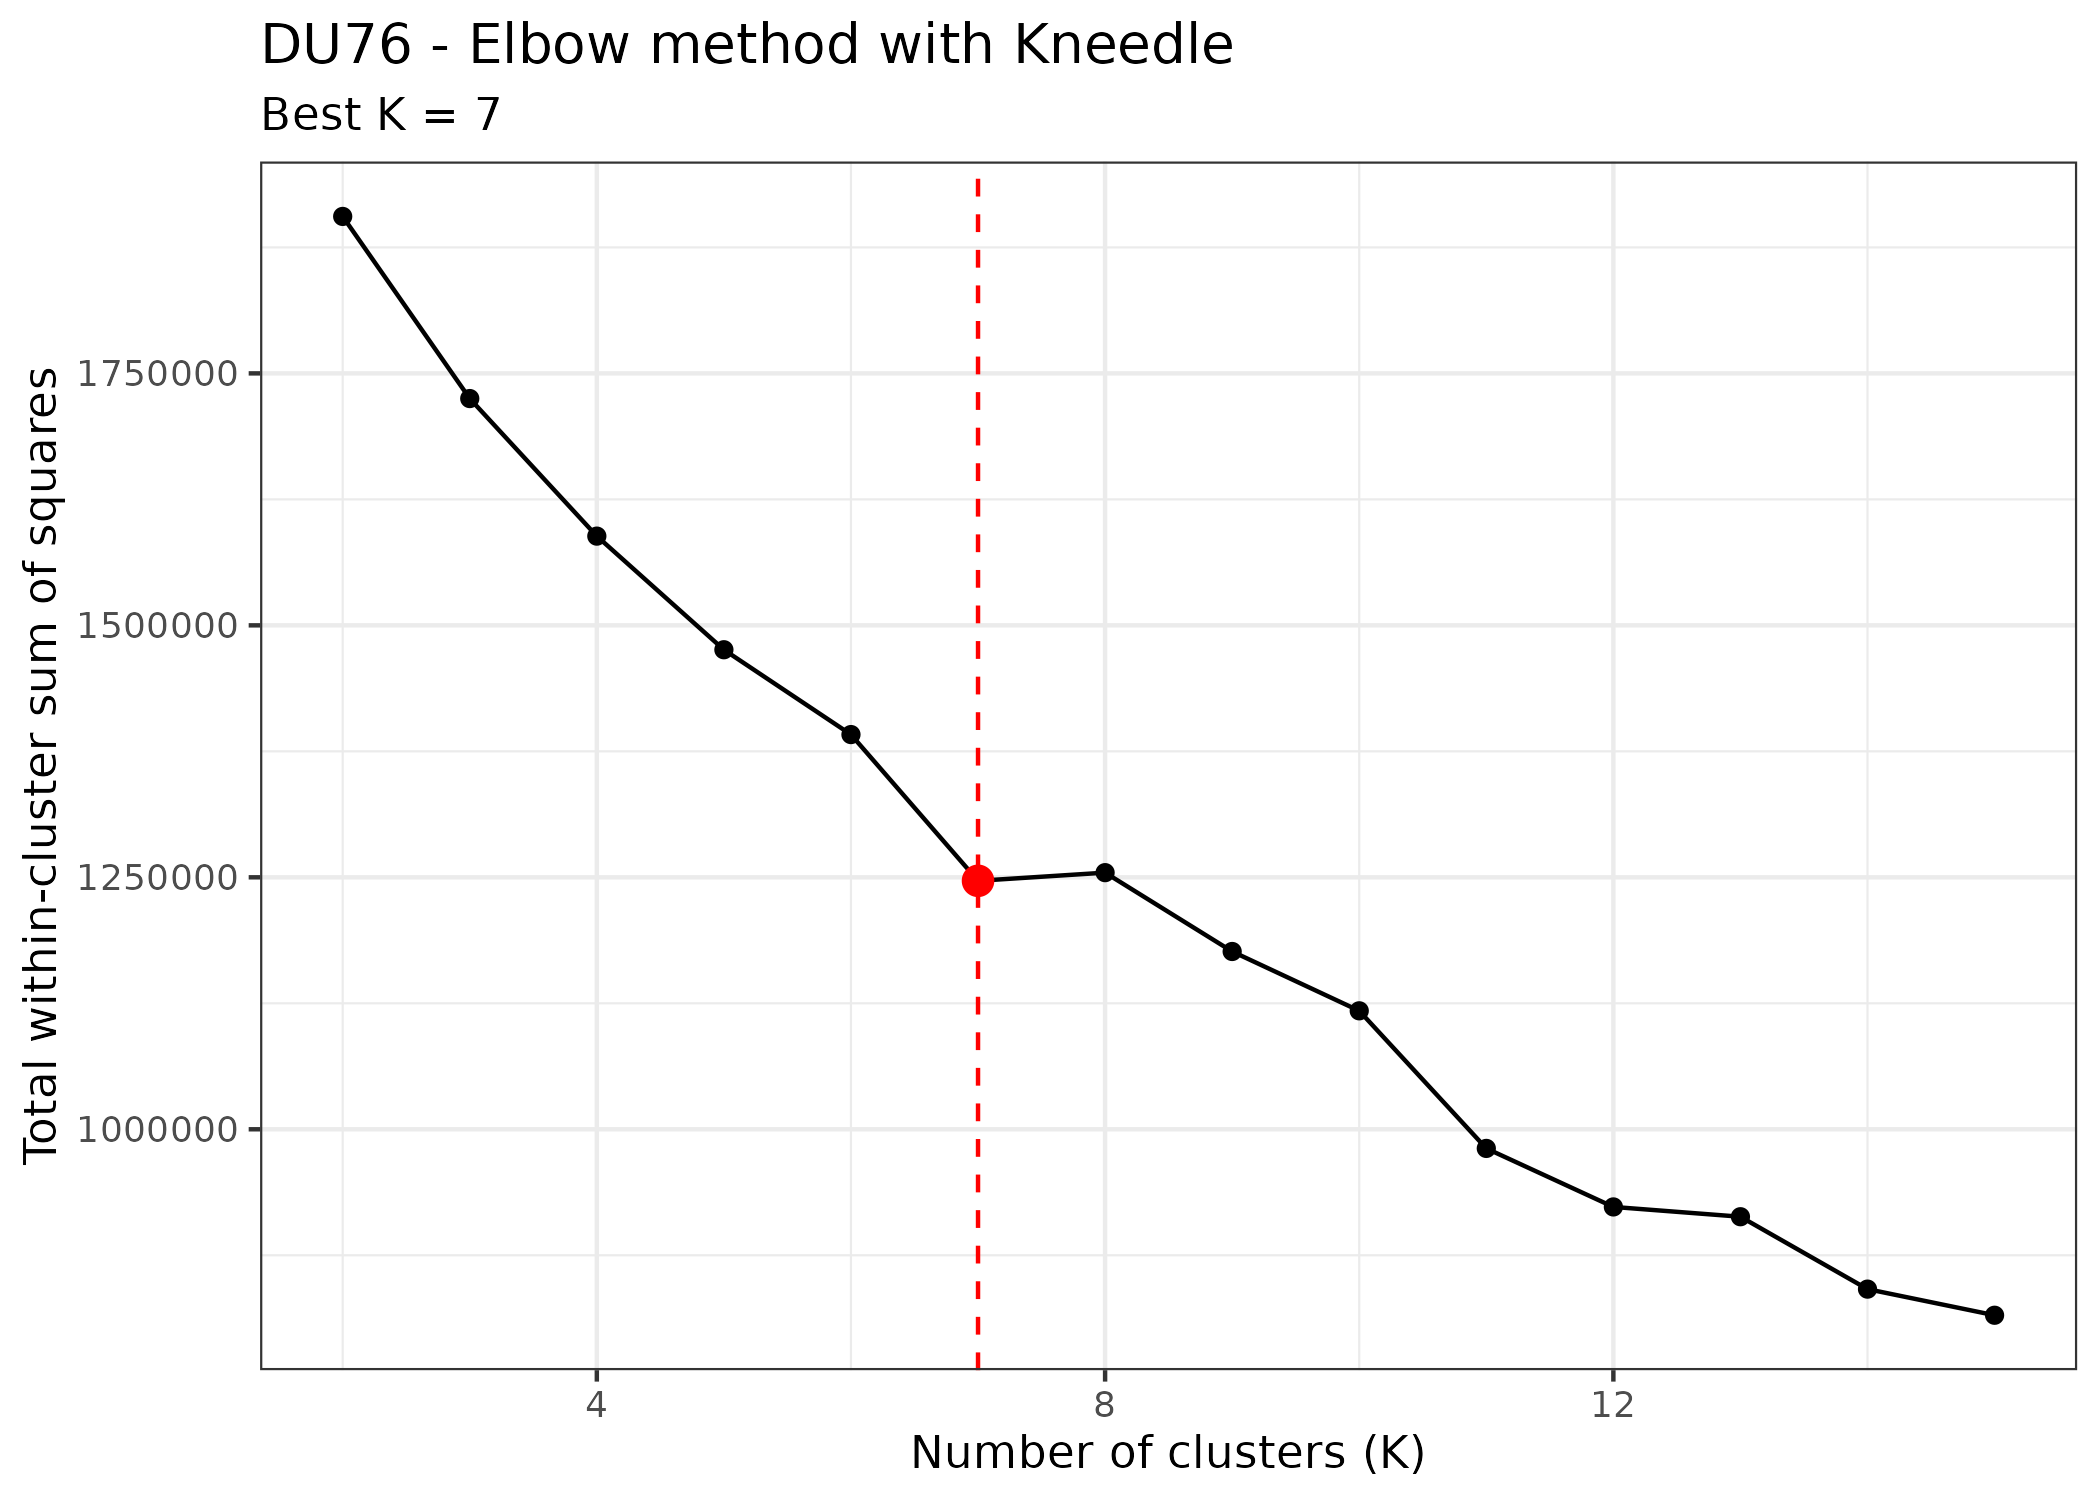
\includegraphics[width=\textwidth]{images/Elbow_Kneedle_DU76.png}
    \caption{Elbow method plot used to determine the optimal number of clusters (K) for the DU76 sample based on the total within-cluster sum of squares (WCSS). The Kneedle algorithm identified K=7 as the optimal clustering solution, corresponding to the point where increasing the number of clusters yields diminishing reductions in intra-cluster variability. The red dashed line and highlighted point indicate the selected elbow point.}
\end{figure} 

\begin{figure}[H]
    \centering
    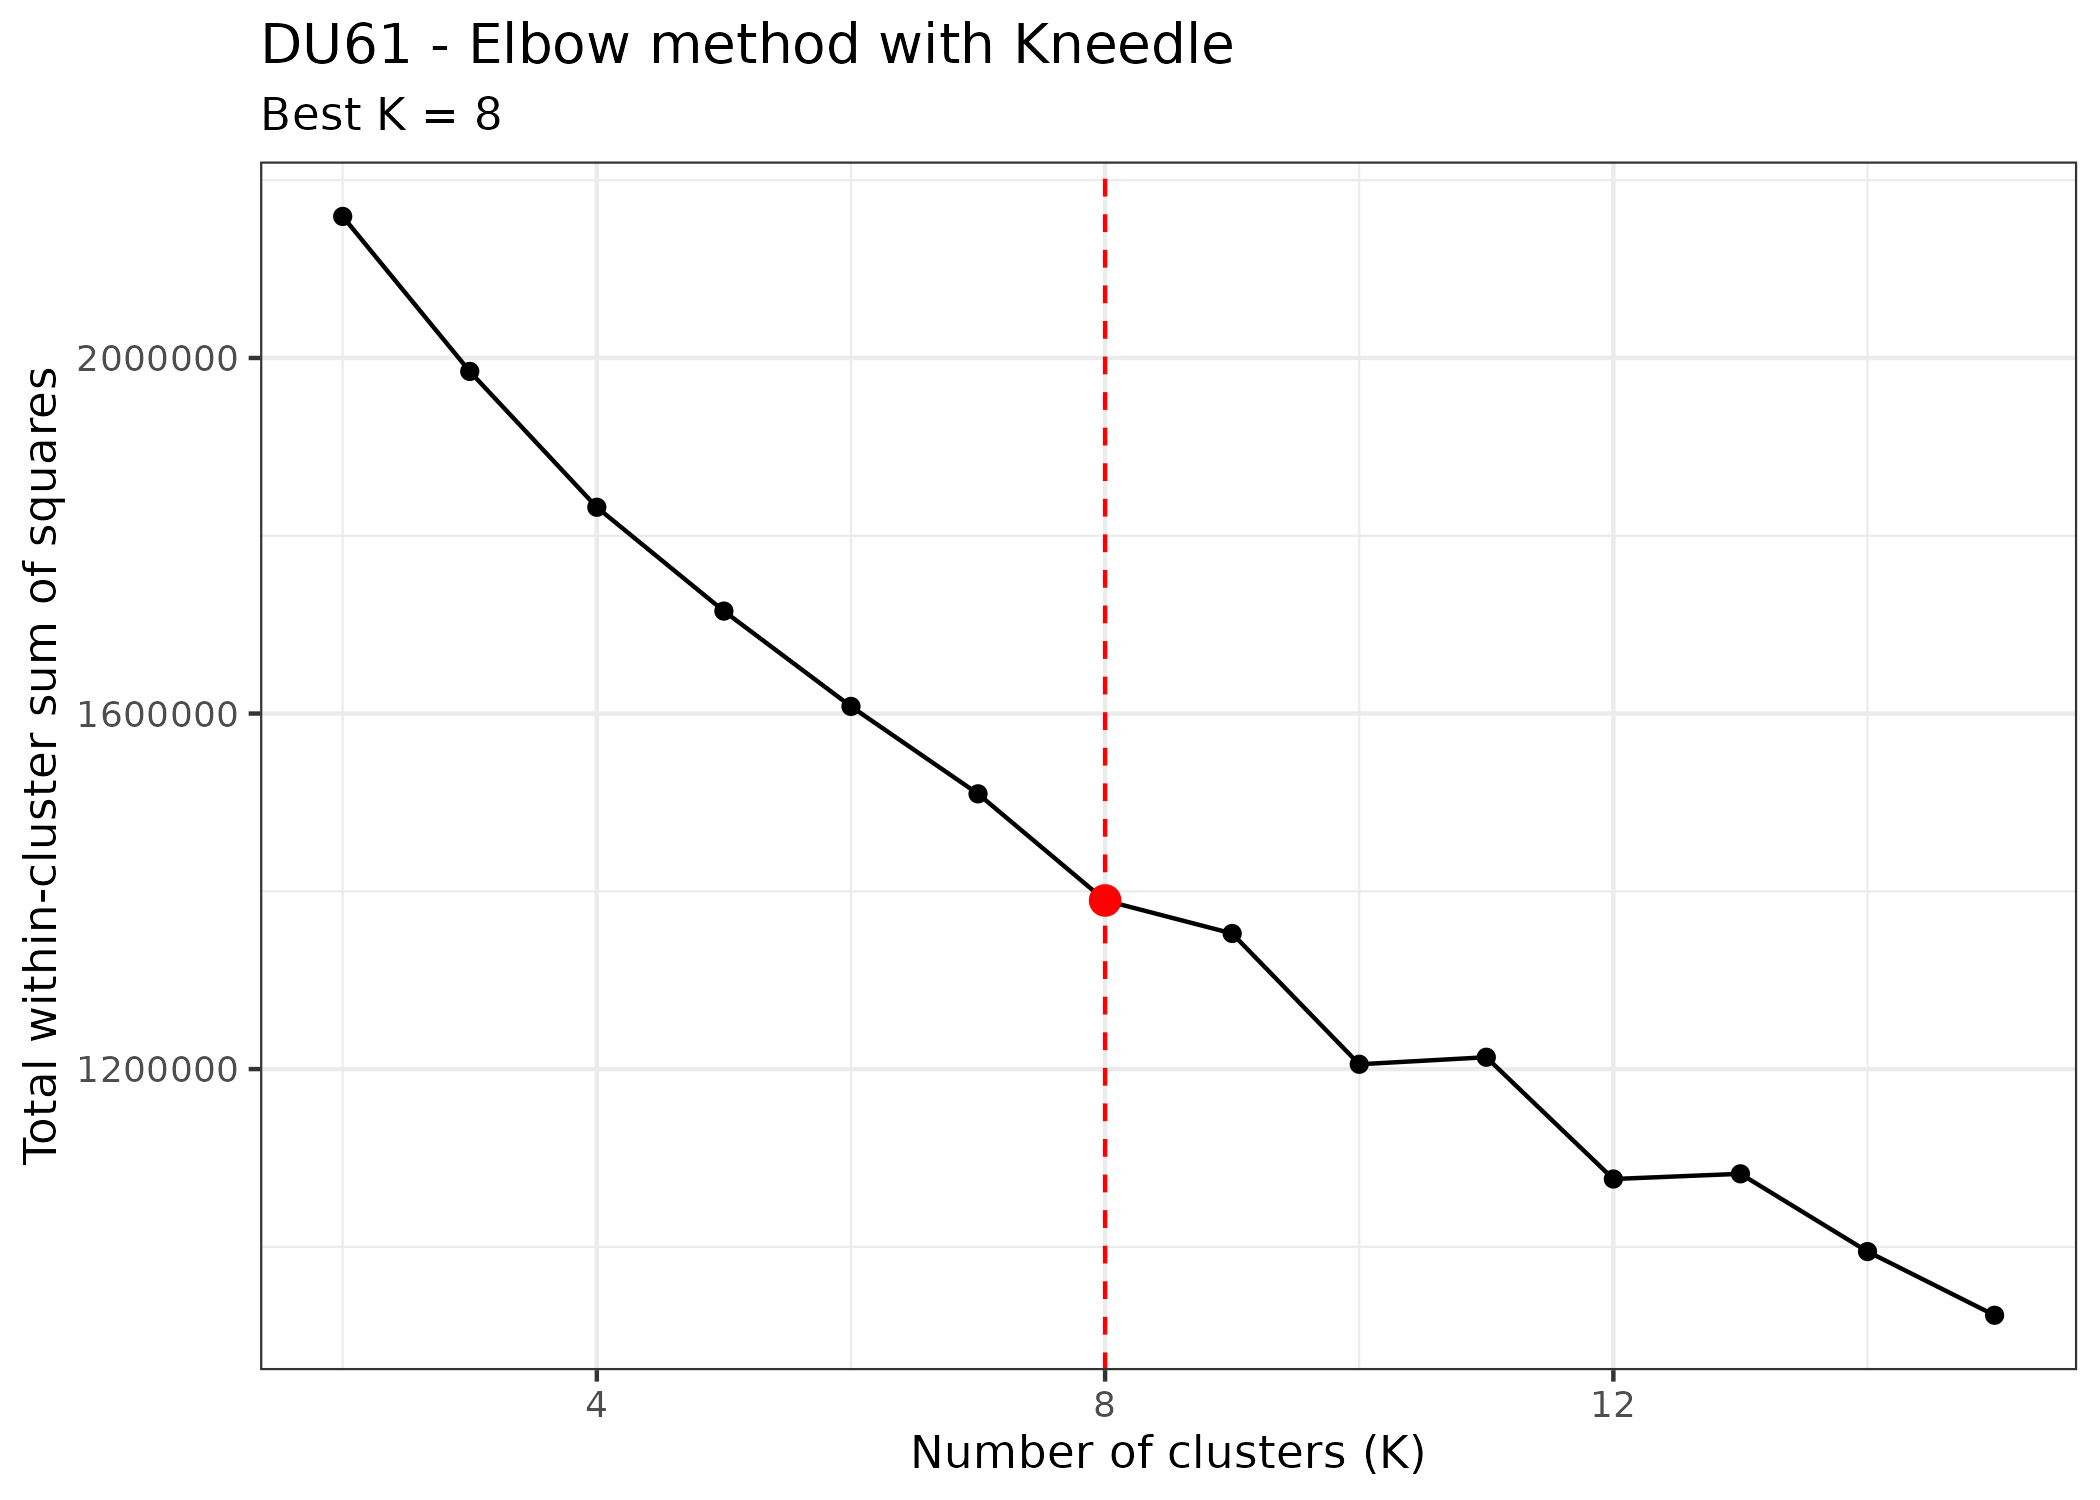
\includegraphics[width=\textwidth]{images/Elbow_Kneedle_DU61.png}
    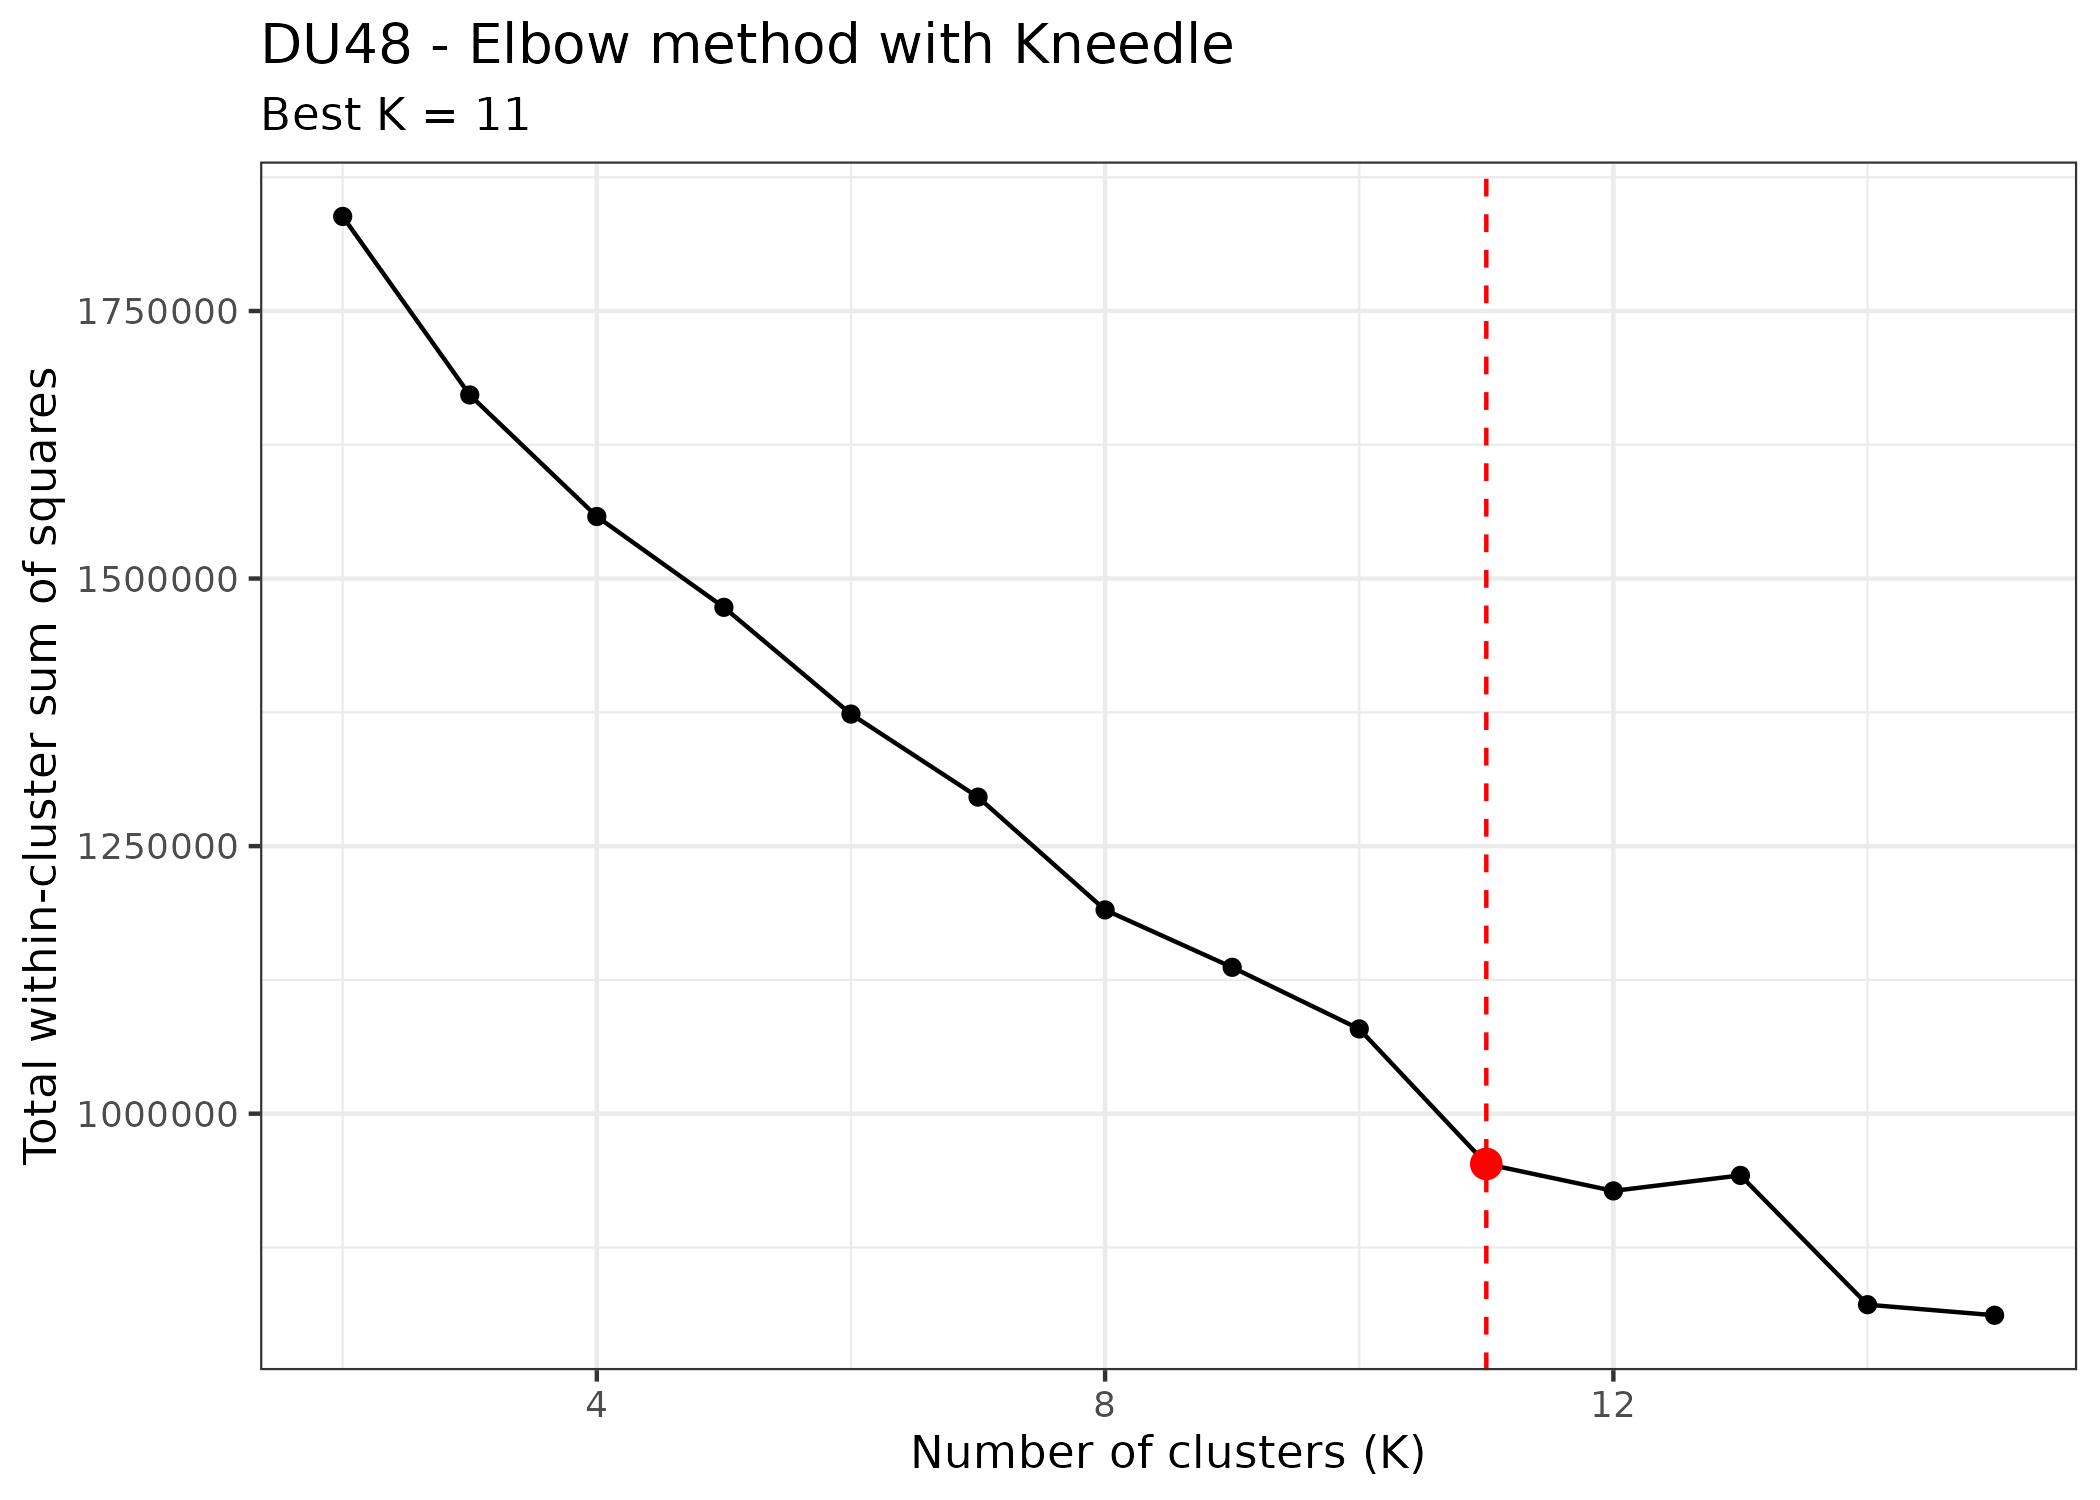
\includegraphics[width=\textwidth]{images/Elbow_Kneedle_DU48.png}
    \caption{Elbow method plot used to determine the optimal number of clusters (K) for DU61 (the first one) and DU46 (the second one) samples based on the total within-cluster sum of squares (WCSS). Example of other K selected by the Kneedle algorithm. The red dashed line and highlighted point indicate the selected elbow point in both images.}
\end{figure} 

Plotting the identified neighbourhood communities across the tissue section provides a direct visualization of biologically meaningful spatial regions within the tumour microenvironment. These spatial communities may indicate enrichment for specific cell types. The spatial organization of stromal, epithelial, and immune-associated communities is biologically relevant, as it may influence local cell-cell interactions, immune infiltration, and ultimately therapeutic response. Consequently, in ST, both statistical composition and spatial localization must be considered to obtain biologically meaningful conclusions.

\begin{figure}[H]
    \centering
    
\includegraphics[width=\textwidth]{images/Spatial_Neighbourhood_K11_DU48.png}
    \caption{Spatial representation of neighbourhood analysis in sample DU53. The left panel shows the spatial distribution of annotated cell types across the tissue section, while the right panel displays the cellular communities identified through K-means clustering based on local neighborhood composition (K=6).}
    \labfig{Communities_plot_48}
\end{figure} 

Sample DU48 presented a partial response following DUTRENEO treatment, with residual tumour still detected in the patient. This indicates that the treatment reduced the tumour burden but did not completely eliminate the disease, suggesting that the tumour may have regressed or disappeared in some regions while persisting, reappearing, or remaining detectable in others. Figure \reffig{Communities_plot_48} illustrates the spatial distribution of annotated cell types and the corresponding neighbourhood-defined cellular communities. The left panel represents the original cell type annotations obtained after cell annotation, whereas the right panel shows the neighbourhood communities identified through K-means clustering based on local cellular composition. Distinct spatially organized regions were identified within the tumour microenvironment, indicating structured cellular organization rather than random cellular distribution. More specifically, the communities represented in white in both panels appeared to correspond to epithelial-dominated regions and potentially tumour-associated areas, as these cells were annotated as epithelial by SingleR and subsequently grouped into the same neighbourhood-defined community (cluster 6). In addition, smooth muscle cells were clearly distinguished from the remaining cell types (the grey cluster numbered 10 on communities plot), while endothelial-rich regions (the green cluster numbered 7 on communities plot) were also visually identifiable.

\begin{figure}[H]
    \centering
    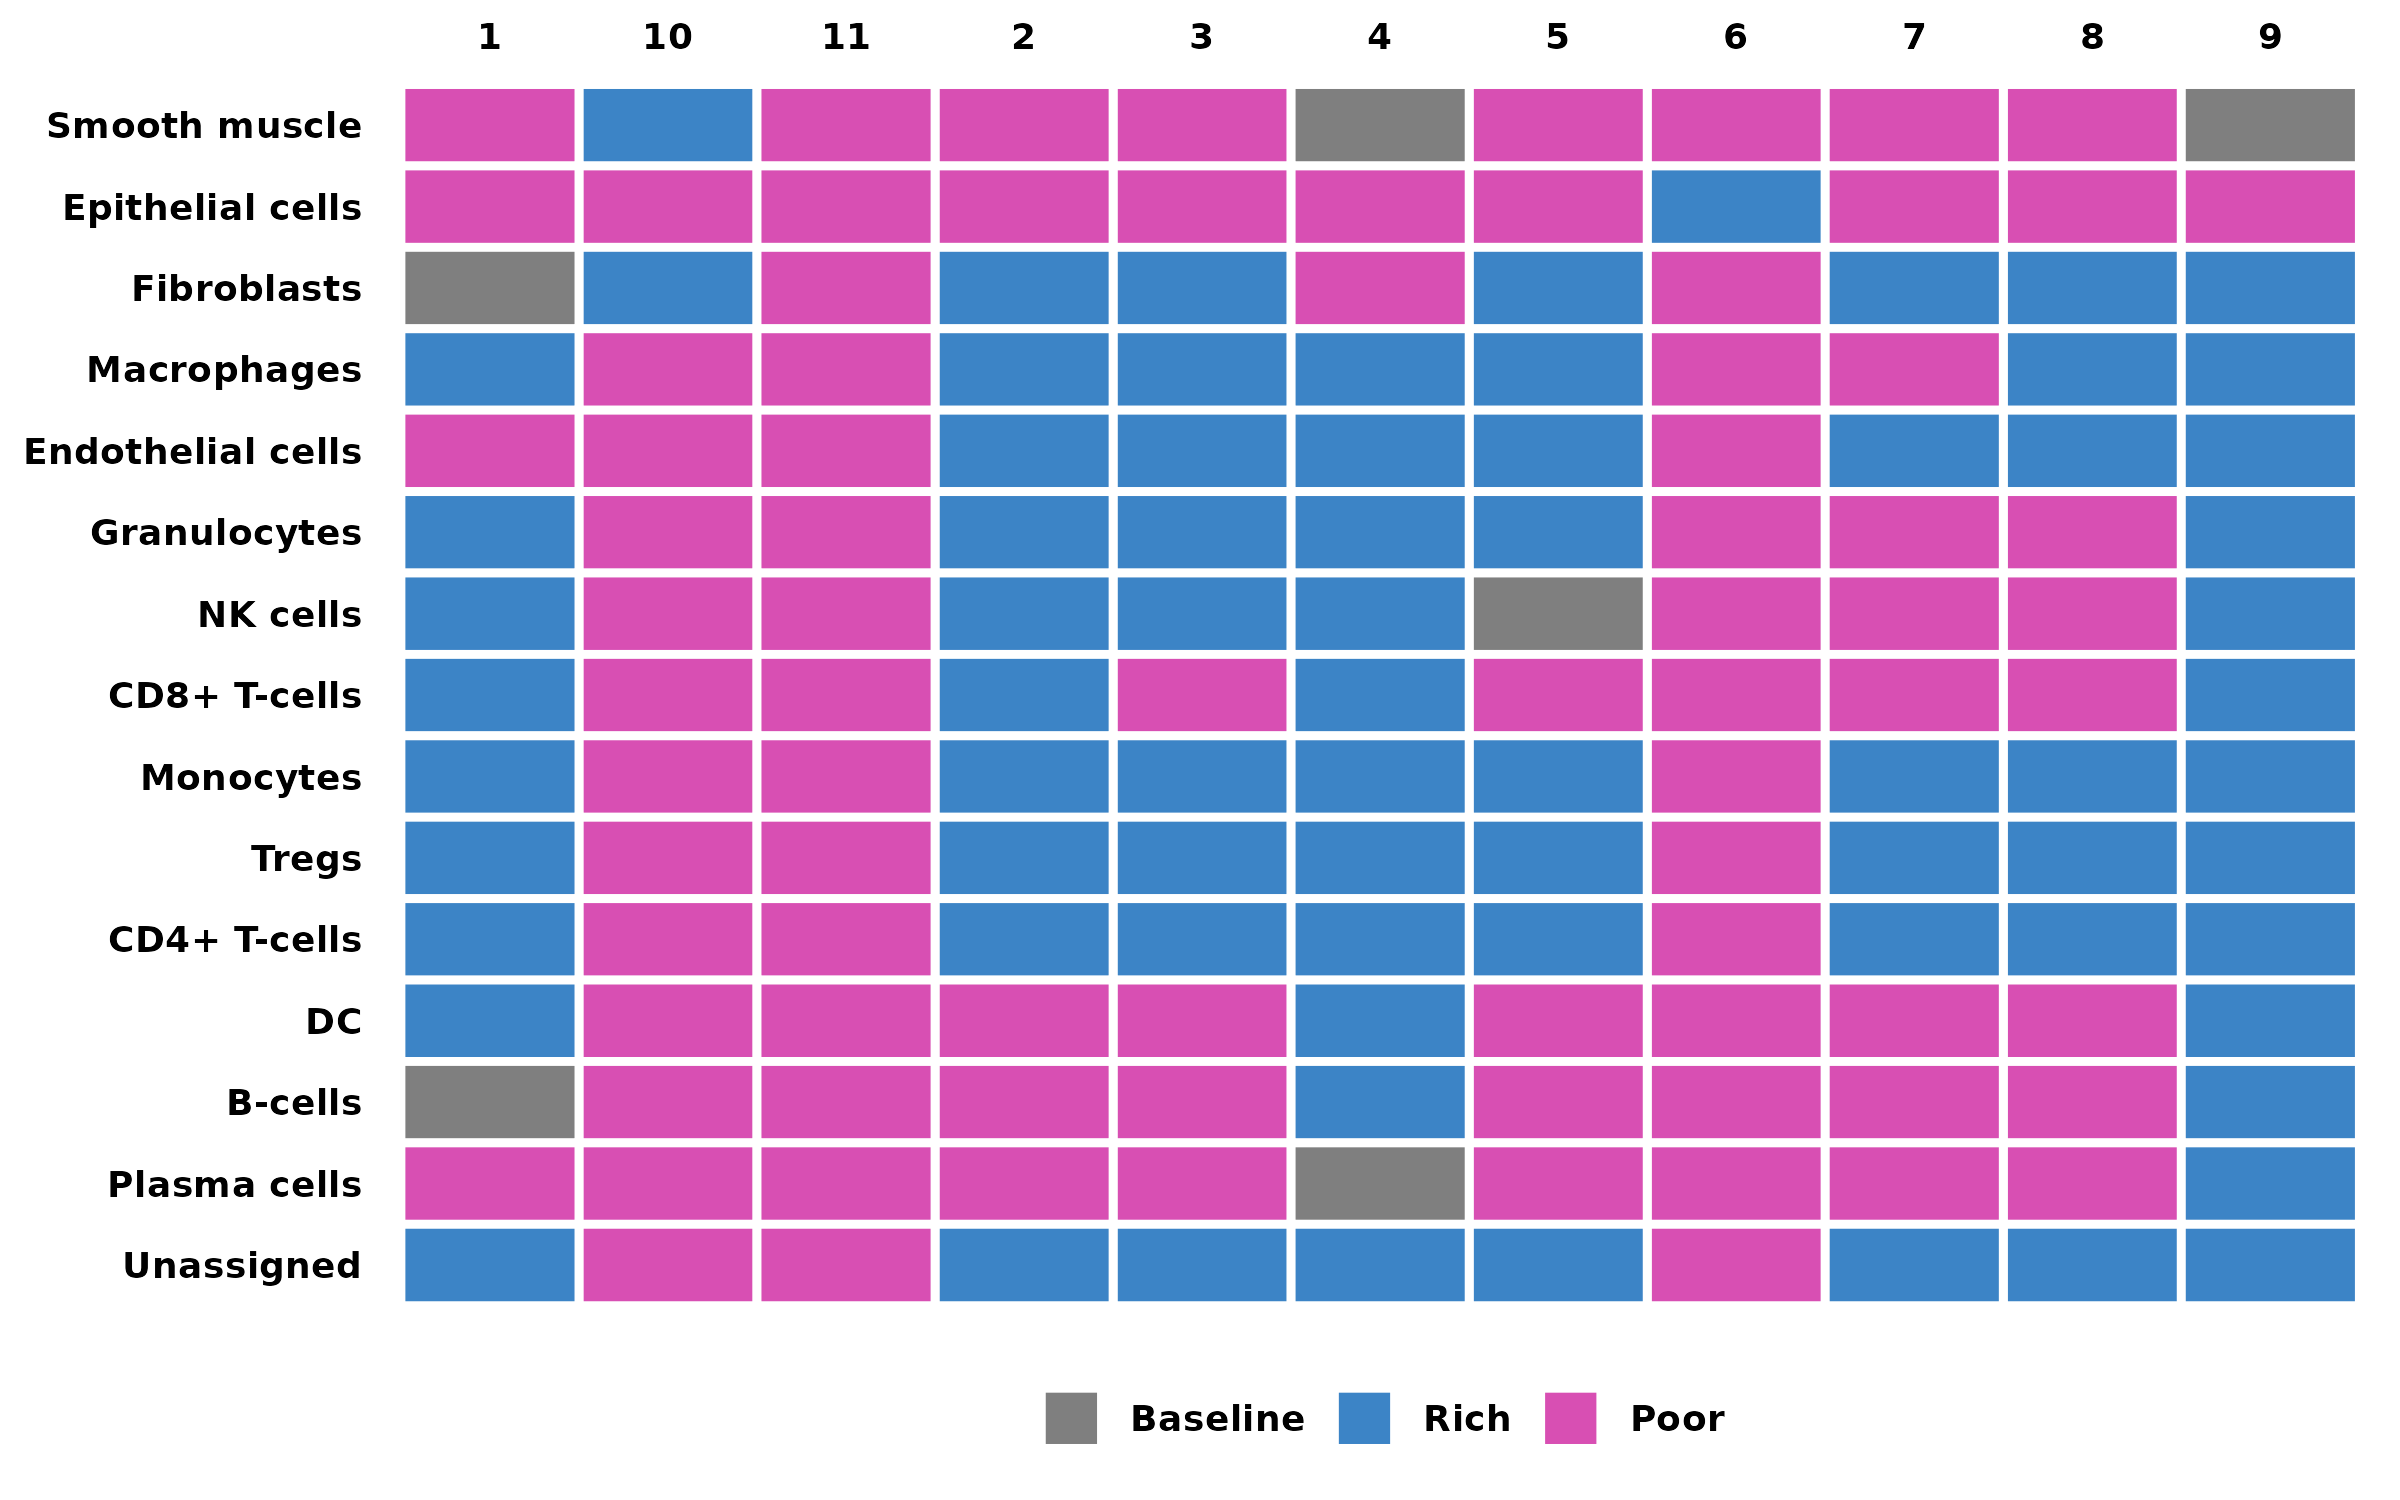
\includegraphics[width=\textwidth]{images/Community_RichPoor_Heatmap_DU48.png}
    \caption{Enrichment and depletion analysis of cell types across the six neighbourhood-defined communities identified in sample DU48. Each column represents a cellular community, while each row corresponds to an annotated cell type. Communities were classified as “rich” (blue), “neutral” (grey), or “poor” (pink) according to the relative abundance of each cell type compared with the remaining communities within the sample. The heatmap highlights the heterogeneous cellular composition of the tumour microenvironment and reveals distincts spatial communities.}
    \labfig{Communities_hetmap_DU48}
\end{figure}

To further characterize the biological identity of each neighbourhood-defined community, enrichment and depletion analyses were performed for all annotated cell types (\reffig{Communities_hetmap_DU48}). Communities were classified as ``rich'', ``neutral'', or ``poor'' depending on whether a given cell type was overrepresented, present at baseline levels, or underrepresented relative to the remaining communities within the same sample. For instance, a fibroblast-rich community corresponds to a spatial region containing a higher proportion of fibroblasts relative to the remaining communities, whereas fibroblast-poor communities contain comparatively fewer fibroblasts. The analysis confirmed that cluster 6 was strongly enriched for epithelial cells while depleted for the remaining cell populations, suggesting that this community was predominantly epithelial in composition. Cluster 10 showed enrichment for smooth muscle cells together with fibroblasts, indicating a stromal-associated region. In contrast, cluster 7 displayed enrichment for endothelial cells together with fibroblasts, monocytes, regulatory T cells, and CD4+ T cells, demonstrating that visual interpretation alone was insufficient to fully characterize the community composition. Furthermore, immune-associated enriched communities appeared spatially localized near tumour-associated regions, potentially reflecting ongoing anti-tumour immune activity. These findings are consistent with the metadata associated with DU48, in which the DUTRENEO treatment produced a partial therapeutic response. Overall, the results suggest that the neighbourhood analysis pipeline successfully identified biologically coherent spatial communities.

Another example is sample DU61, presented a complete response despite the detection of residual tumour-associated transcriptomic alterations. In Figure \reffig{Communities_plot_61}, a spatially localized epithelial-rich region can be observed, represented in dark green in the annotation panel and orange in the community panel (cluster 2). This region potentially corresponds to residual tumour-associated epithelial cells. The objective of this thesis is not to distinguish malignant from non-malignant epithelial cells directly, but rather to identify spatial regions potentially associated with tumour persistence in order to facilitate future analyses.

\begin{figure}[H]
    \centering
    \includegraphics[width=\textwidth]{images/Spatial_Neighbourhood_K8_DU61.png}
    \caption{Spatial representation of neighbourhood analysis in sample DU61. The left panel shows the spatial distribution of annotated cell types across the tissue section, while the right panel displays the cellular communities identified through K-means clustering based on local neighborhood composition (K=8).}
    \labfig{Communities_plot_61}
\end{figure} 

The enrichment analysis shown in Figure \reffig{Communities_hetmap_DU61} confirmed that cluster 2 was enriched almost exclusively for epithelial cells, whereas cluster 4 was enriched for smooth muscle cells and fibroblasts. Importantly, cluster 5 was enriched for immune-associated cell populations and appeared spatially distributed between stromal and epithelial-rich regions. Given that DU61 exhibited a complete response with the standard treatment despite the presence of residual transcriptomic alterations, these observations raise the possibility that immune-associated communities may have successfully infiltrated tumour-associated regions despite the surrounding stromal organization. However, additional immune-expression and statistical analyses would be required in order to draw definitive biological conclusions. 

\begin{figure}[H]
    \centering
    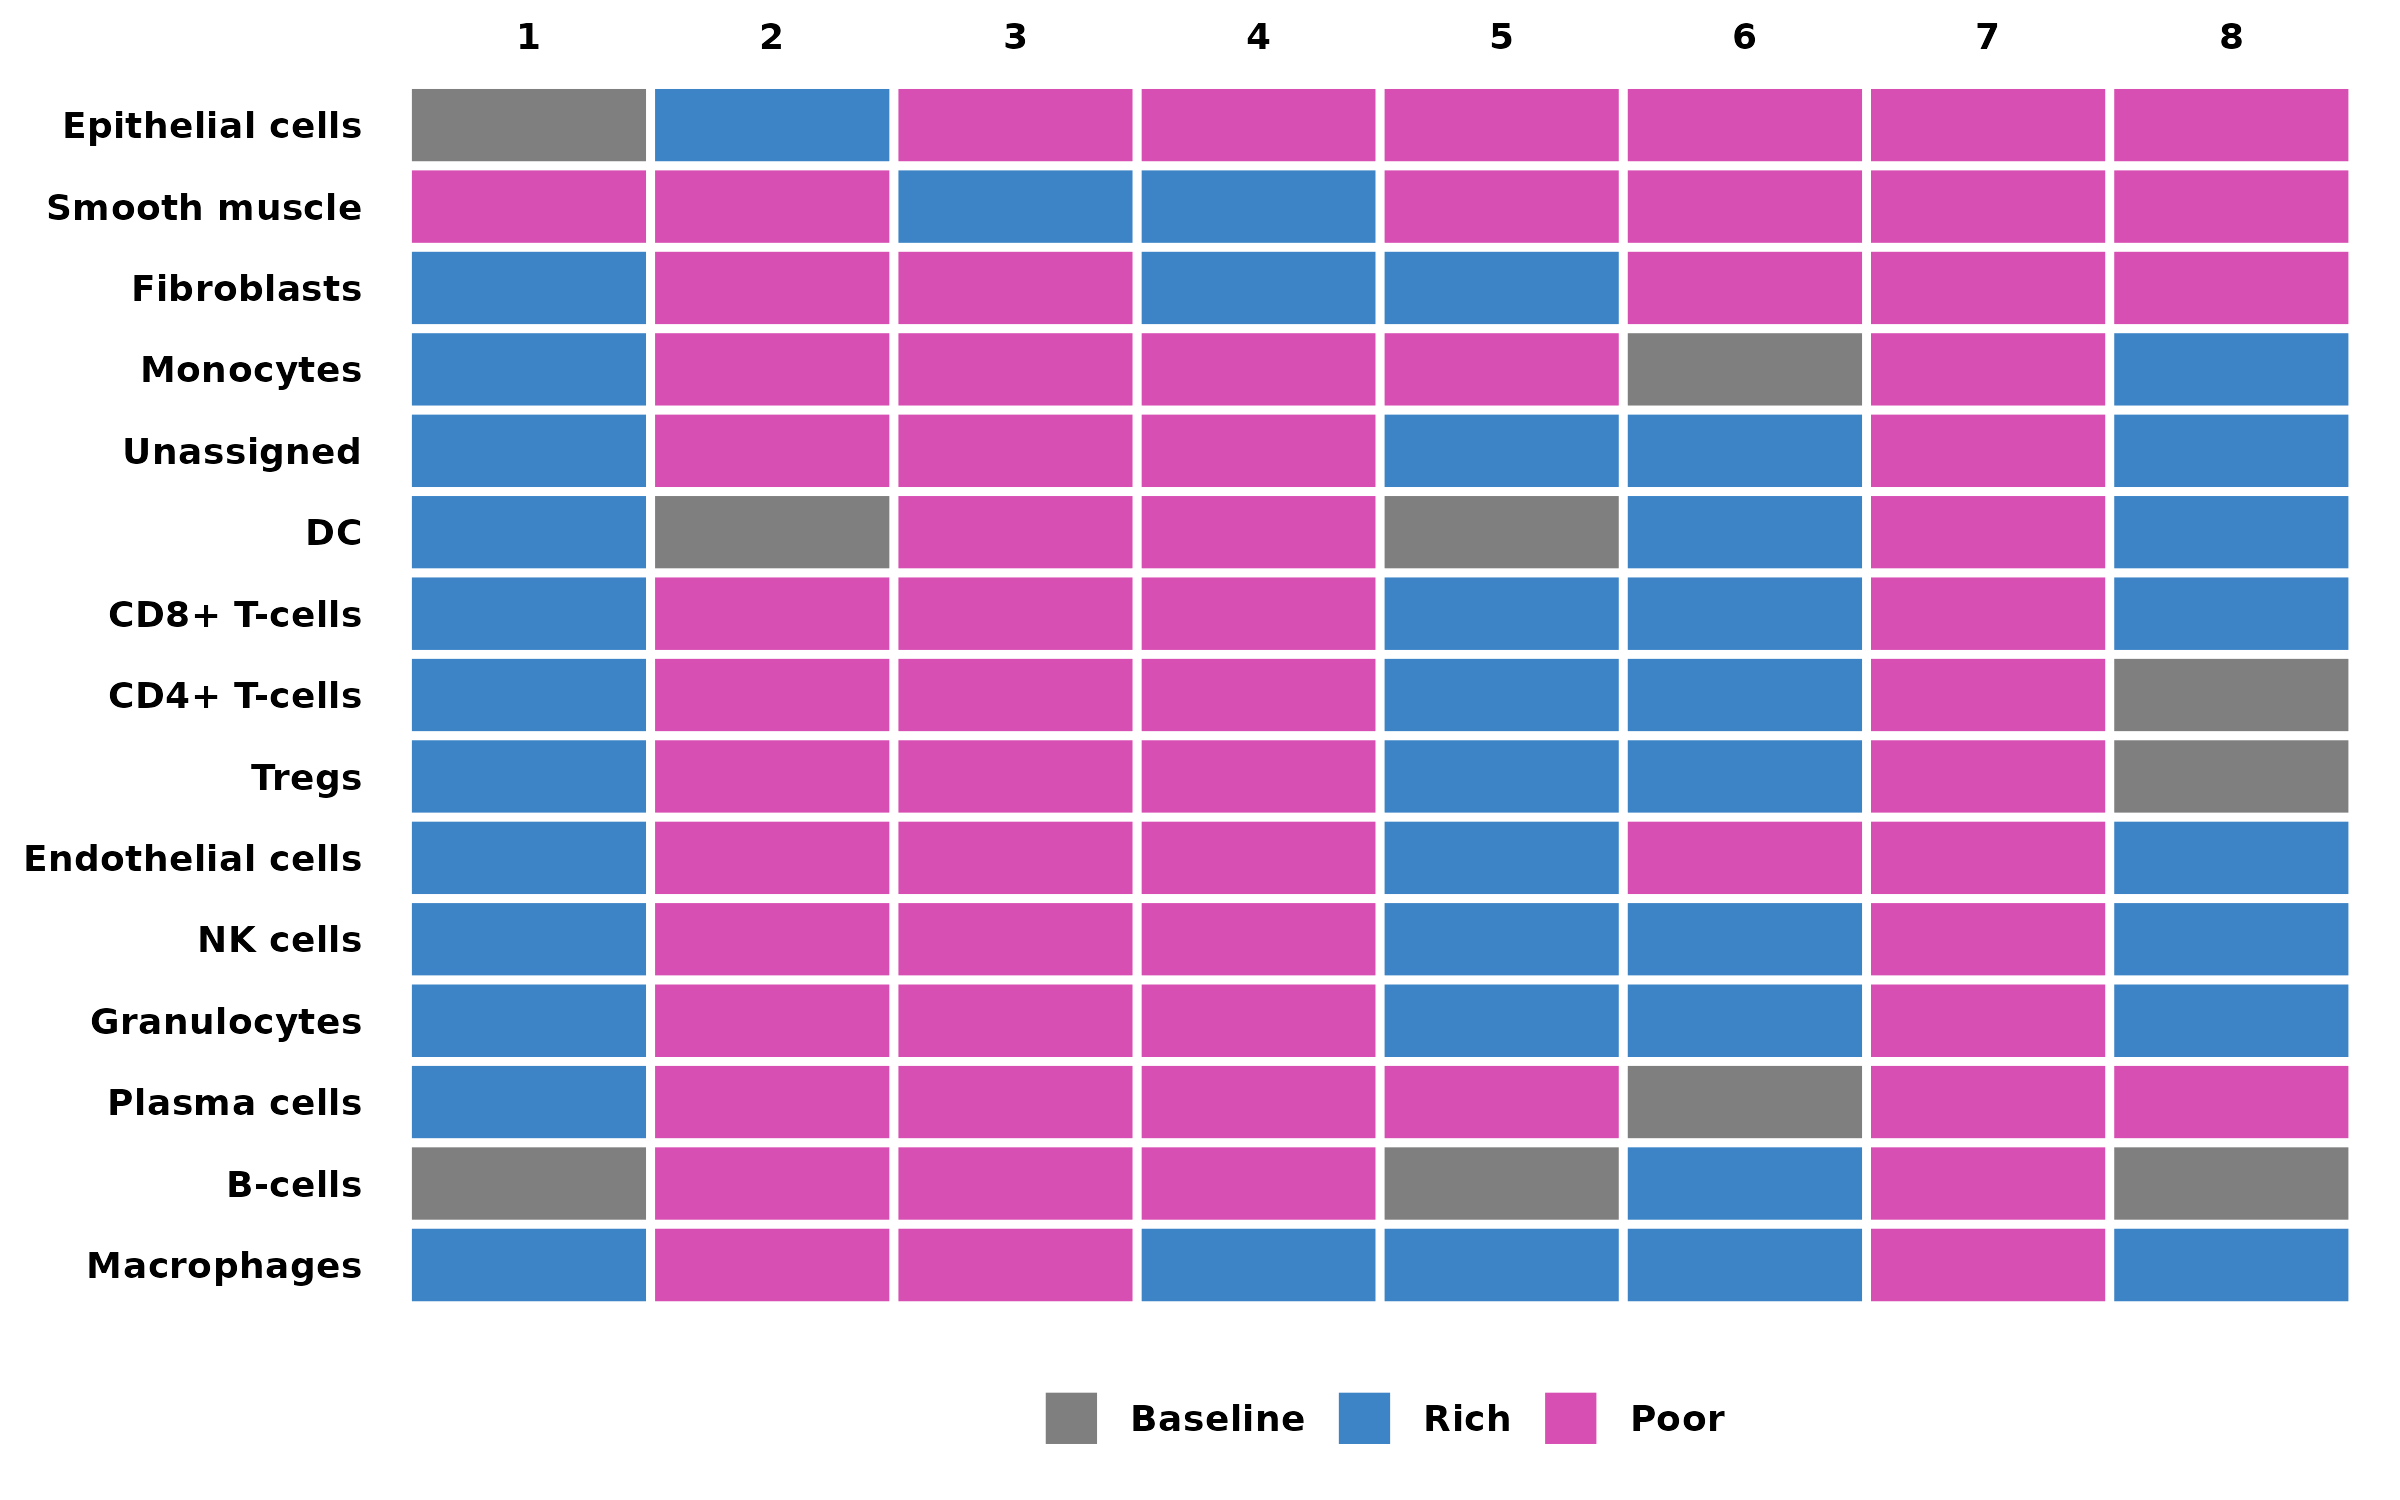
\includegraphics[width=\textwidth]{images/Community_RichPoor_Heatmap_DU61.png}
    \caption{Enrichment and depletion analysis of cell types across the six neighbourhood-defined communities identified in sample DU61. Each column represents a cellular community, while each row corresponds to an annotated cell type. Communities were classified as “rich” (blue), “neutral” (grey), or “poor” (pink) according to the relative abundance of each cell type compared with the remaining communities within the sample. The heatmap highlights the heterogeneous cellular composition of the tumour microenvironment and reveals distincts spatial communities.}
    \labfig{Communities_hetmap_DU61}
\end{figure}

The final example corresponds to sample DU76, in which no detectable tumour tissue was present. Therefore, if the neighbourhood analysis results are consistent with the clinical metadata, this would further support the validity and robustness of the proposed analytical pipeline across different biological scenarios. In Figure \reffig{Communities_plot_76}, an epithelial-associated region can be observed, highlighted in grey in the annotation panel and grouped into a blue community in the clustering panel. Consequently, it is important to evaluate whether this region is enriched for epithelial cells in the corresponding enrichment matrix. The remaining communities showed patterns similar to those observed in previous samples, including a clearly defined smooth muscle-associated cluster. In addition, several interesting mixed cellular communities were identified by K-means clustering and are represented in green, red, and orange.

\begin{figure}[H]
    \centering
    
\includegraphics[width=\textwidth]{images/Spatial_Neighbourhood_K7_DU76.png}
    \caption{Spatial representation of neighbourhood analysis in sample DU53. The left panel shows the spatial distribution of annotated cell types across the tissue section, while the right panel displays the cellular communities identified through K-means clustering based on local neighborhood composition (K=7).}
    \labfig{Communities_plot_76}
\end{figure} 

In Figure \reffig{Communities_hetmap_DU76}, the region that visually appeared endothelial-enriched was shown to correspond instead to a mixed community enriched for multiple cell types, consistent with the tumour-free metadata associated with this sample. The smooth muscle-associated cluster was correctly identified, while the green, red, and orange communities also corresponded to mixed cellular populations. Importantly, these mixed communities displayed enrichment for several immune-associated cell types, potentially indicating active anti-tumour immune responses. Furthermore, very limited fibroblast enrichment was observed between immune-associated and epithelial-associated regions. As DU76 corresponded to the only sample without detectable tumour tissue, these observations may suggest that the DUTRENEO treatment effectively reinforced immune activity without substantial stromal suppression, thereby allowing immune cells to access tumour-associated regions without the presence of a significant physical barrier.

\begin{figure}[H]
    \centering
    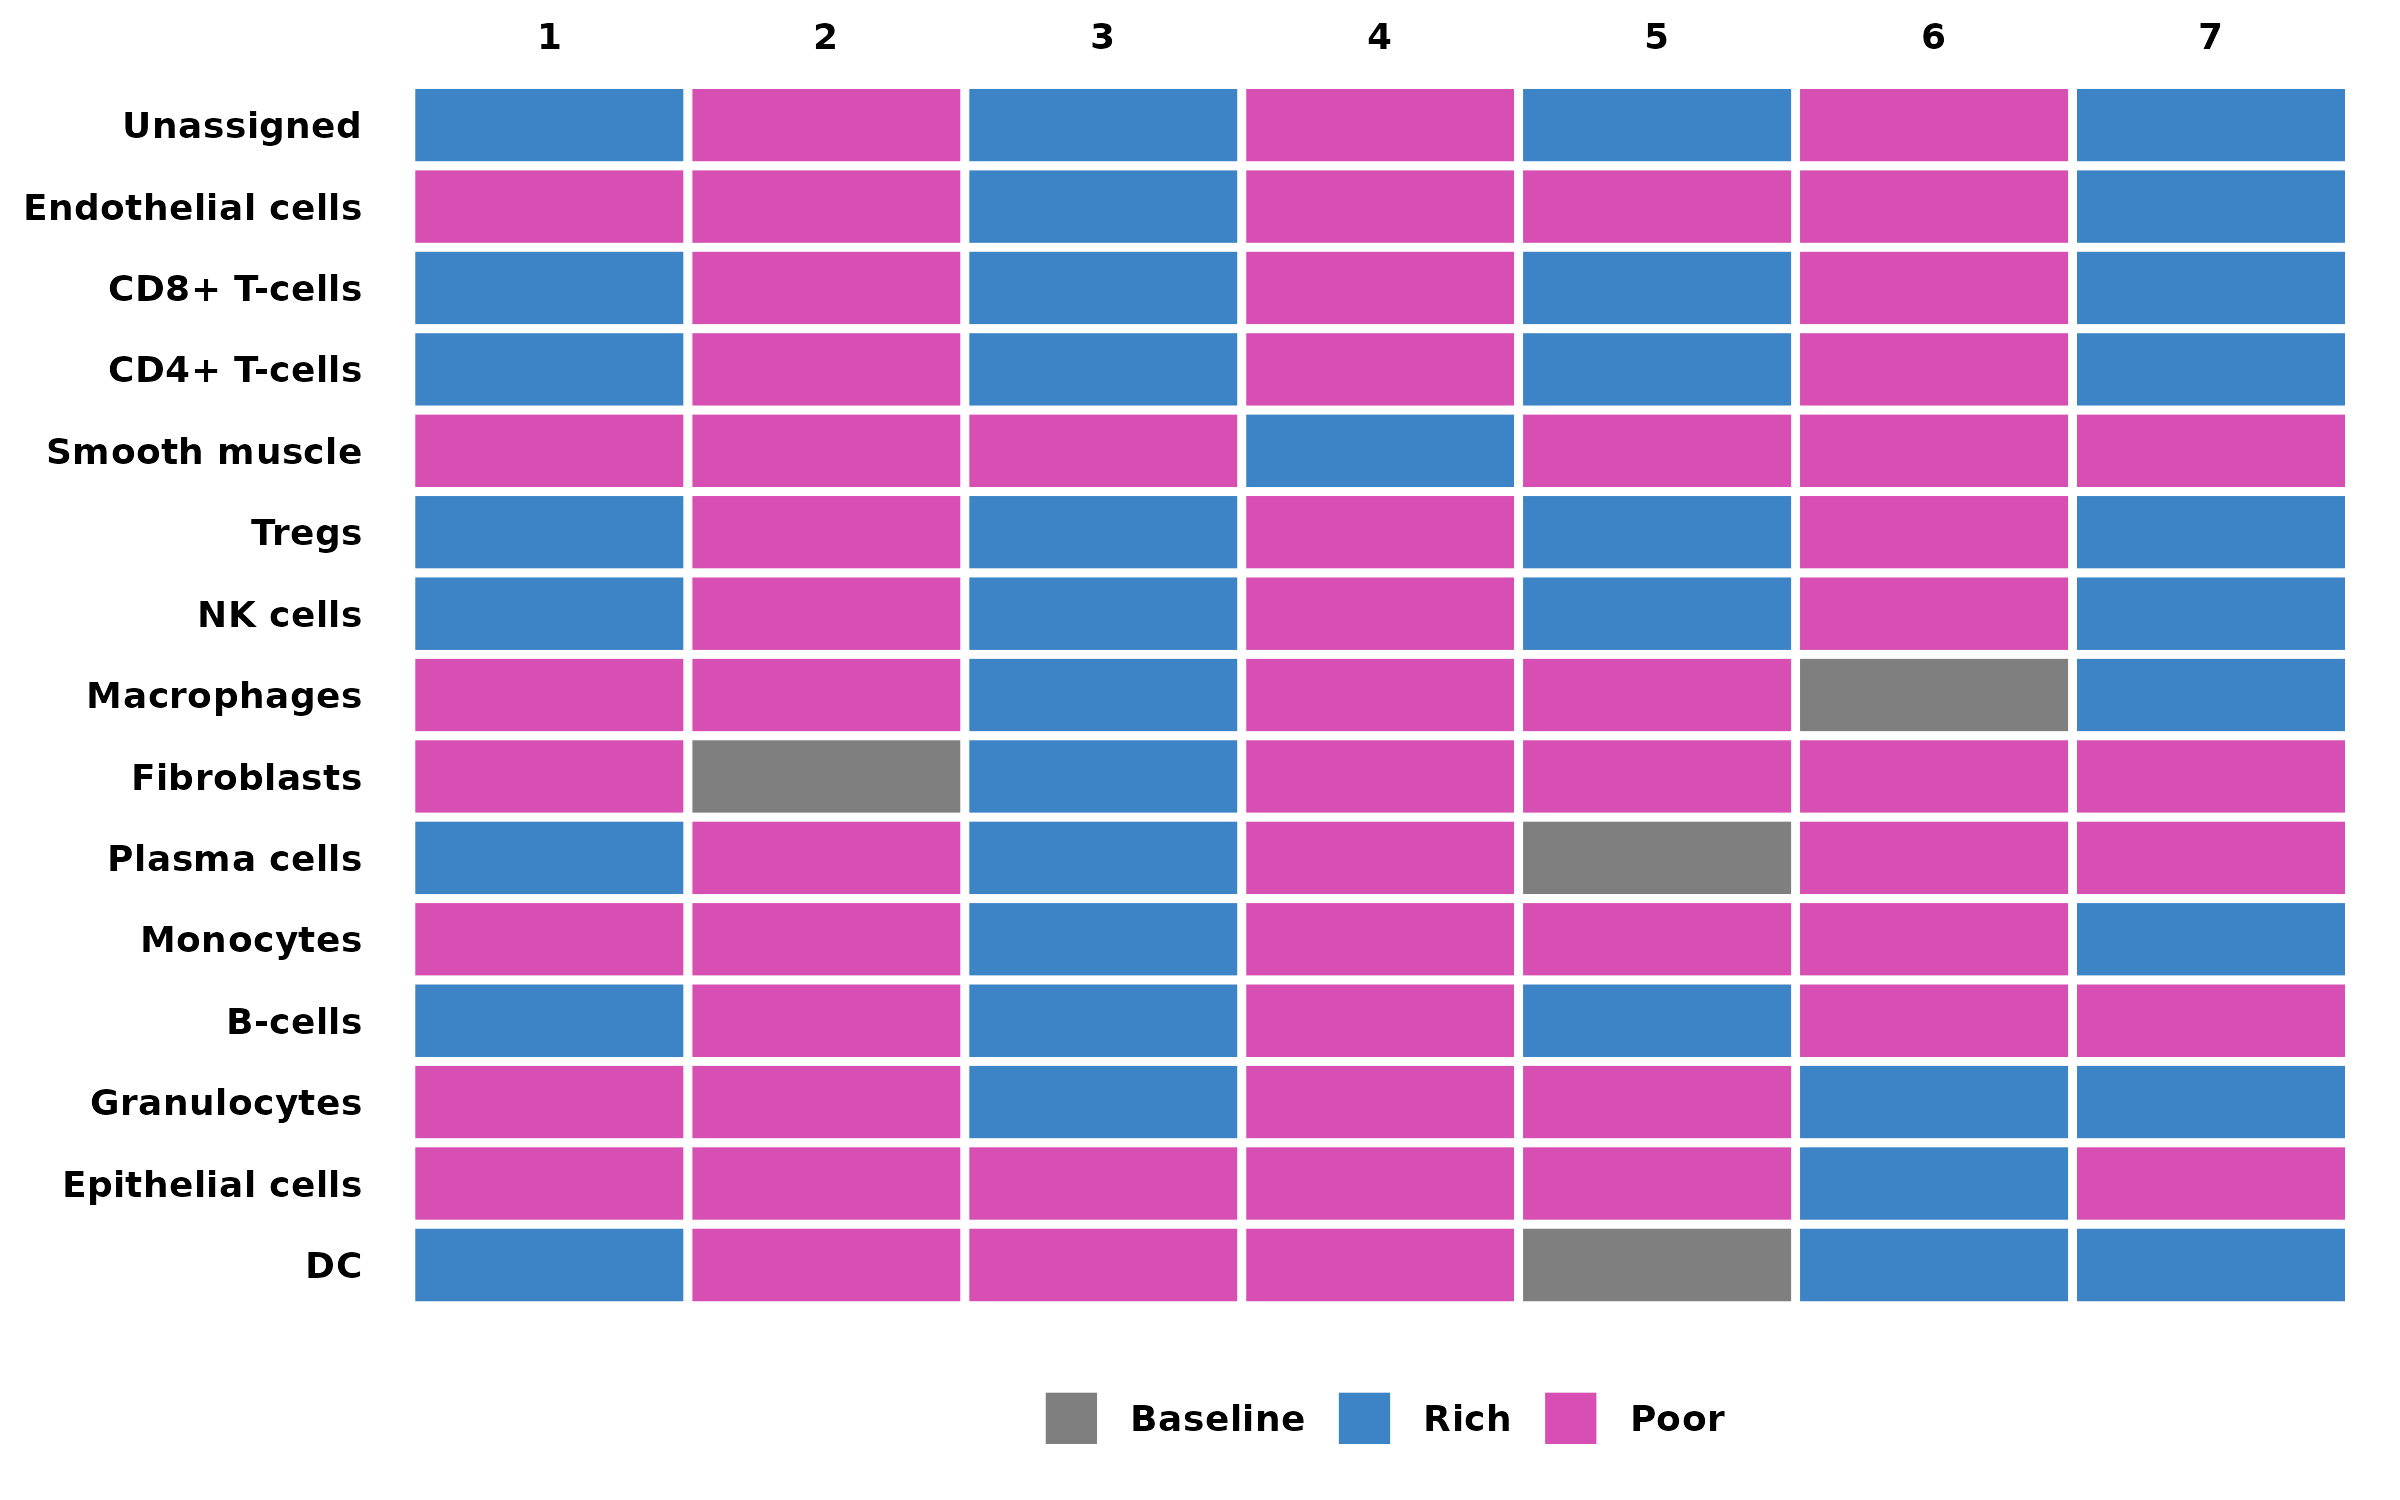
\includegraphics[width=\textwidth]{images/Community_RichPoor_Heatmap_DU76.png}
    \caption{Enrichment and depletion analysis of cell types across the six neighbourhood-defined communities identified in sample DU61. Each column represents a cellular community, while each row corresponds to an annotated cell type. Communities were classified as “rich” (blue), “neutral” (grey), or “poor” (pink) according to the relative abundance of each cell type compared with the remaining communities within the sample. The heatmap highlights the heterogeneous cellular composition of the tumour microenvironment and reveals distincts spatial communities.}
    \labfig{Communities_hetmap_DU76}
\end{figure}


To biologically interpret the enrichment and depletion patterns identified across neighbourhood-defined communities, the spatial distribution of selected ``cell type-rich'' and ``cell type-poor'' communities was projected back onto the original tissue coordinates (\reffig{Rich_Poor_tissue48}). This spatial reconstruction is essential because enrichment analyses alone do not provide information regarding the localization of these communities within the tumour architecture. In sample DU48, epithelial-rich communities appeared highly localized and spatially constrained to well-defined tumour-associated regions, whereas fibroblast-rich and fibroblast-poor communities displayed markedly different spatial distributions across the tissue section. More specifically, fibroblast-enriched regions appeared densely distributed around endothelial-associated and epithelial-associated areas, potentially suggesting that stromal organization may have acted as a physical barrier limiting immune-cell infiltration into tumour-associated regions. This observation may help explain why the treatment achieved only a partial response in this sample. Overall, the organization of these communities demonstrates that tumour microenvironments are not randomly distributed, but instead form structured spatial ecosystems with distinct biological identities.

\begin{figure}[H]
    \centering
    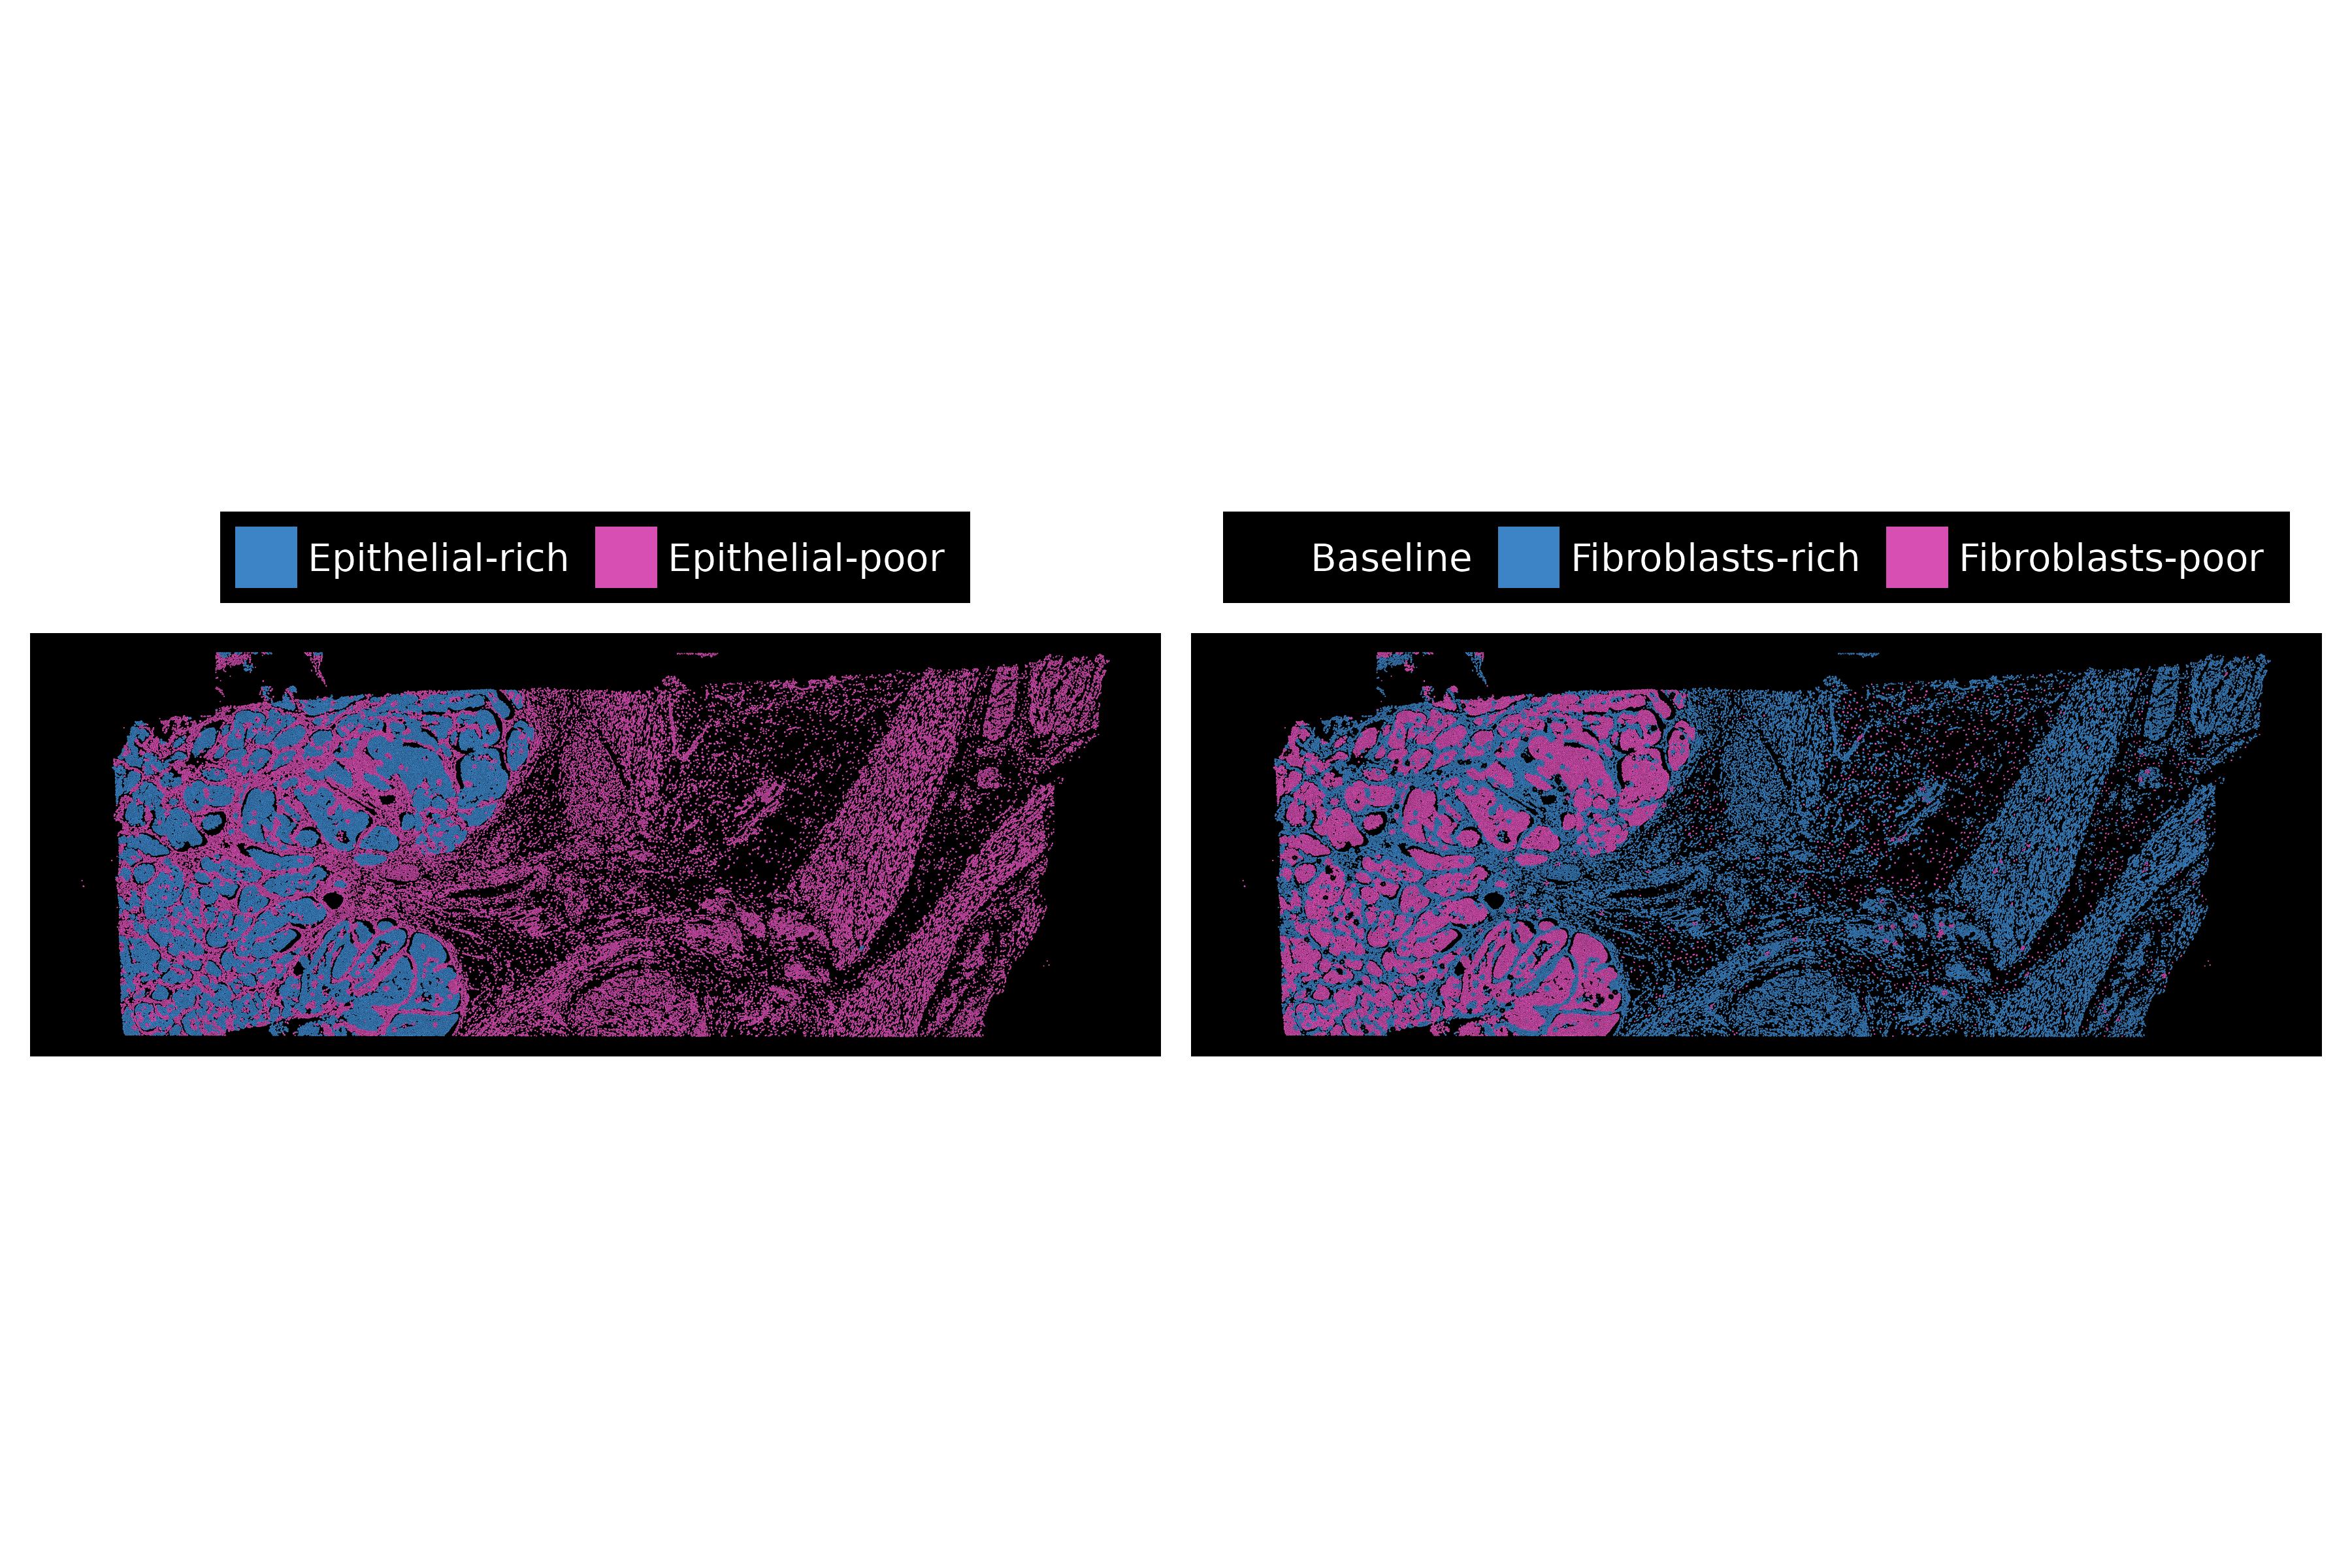
\includegraphics[width=\textwidth]{images/RichPoor_Communities_DU48.png}
    \caption{Spatial distribution of enriched and depleted neighbourhood-defined communities in sample DU48. The left panel shows the localization of epithelial-rich communities, while the right panel displays fibroblast-rich and fibroblast-poor communities projected onto the tissue coordinates.}
    \labfig{Rich_Poor_tissue48}
\end{figure}

This dense fibroblast-associated organization surrounding epithelial-rich, potentially tumour-associated regions was not observed in either the partial-response tumour-free sample (\reffig{Rich_Poor_tissue76}) or the complete-response sample (\reffig{Rich_Poor_tissue61}). In the complete-response sample, although residual malignancy-associated transcriptomic alterations remained detectable in epithelial cells, the fibroblast-rich regions appeared diffusely distributed throughout the tissue rather than densely localized around epithelial-associated areas, as observed in sample DU48. Since this sample underwent conventional chemotherapy treatment, these observations may suggest that therapeutic response depended primarily on direct cytotoxic effects rather than immune-cell infiltration through stromal barriers.

\begin{figure}[H]
    \centering
    
\includegraphics[width=\textwidth]{images/RichPoor_Communities_DU61.png}
    \caption{Spatial distribution of enriched and depleted neighbourhood-defined communities in sample DU61. The left panel shows the localization of epithelial-rich communities, while the right panel displays fibroblast-rich and fibroblast-poor communities projected onto the tissue coordinates.}
    \labfig{Rich_Poor_tissue61}
\end{figure}

The tumour-free sample displayed only a slight more dense fibroblast enriched region within epithelial-poor regions, while the epithelial-enriched region itself showed very limited nearby fibroblast enrichment. These observations may suggest that the DUTRENEO treatment was highly effective within this tissue section, as no substantial stromal barrier appeared to restrict the access of the reinforced and non-suppressed immune system to tumour-associated regions.

\begin{figure}[H]
    \centering
    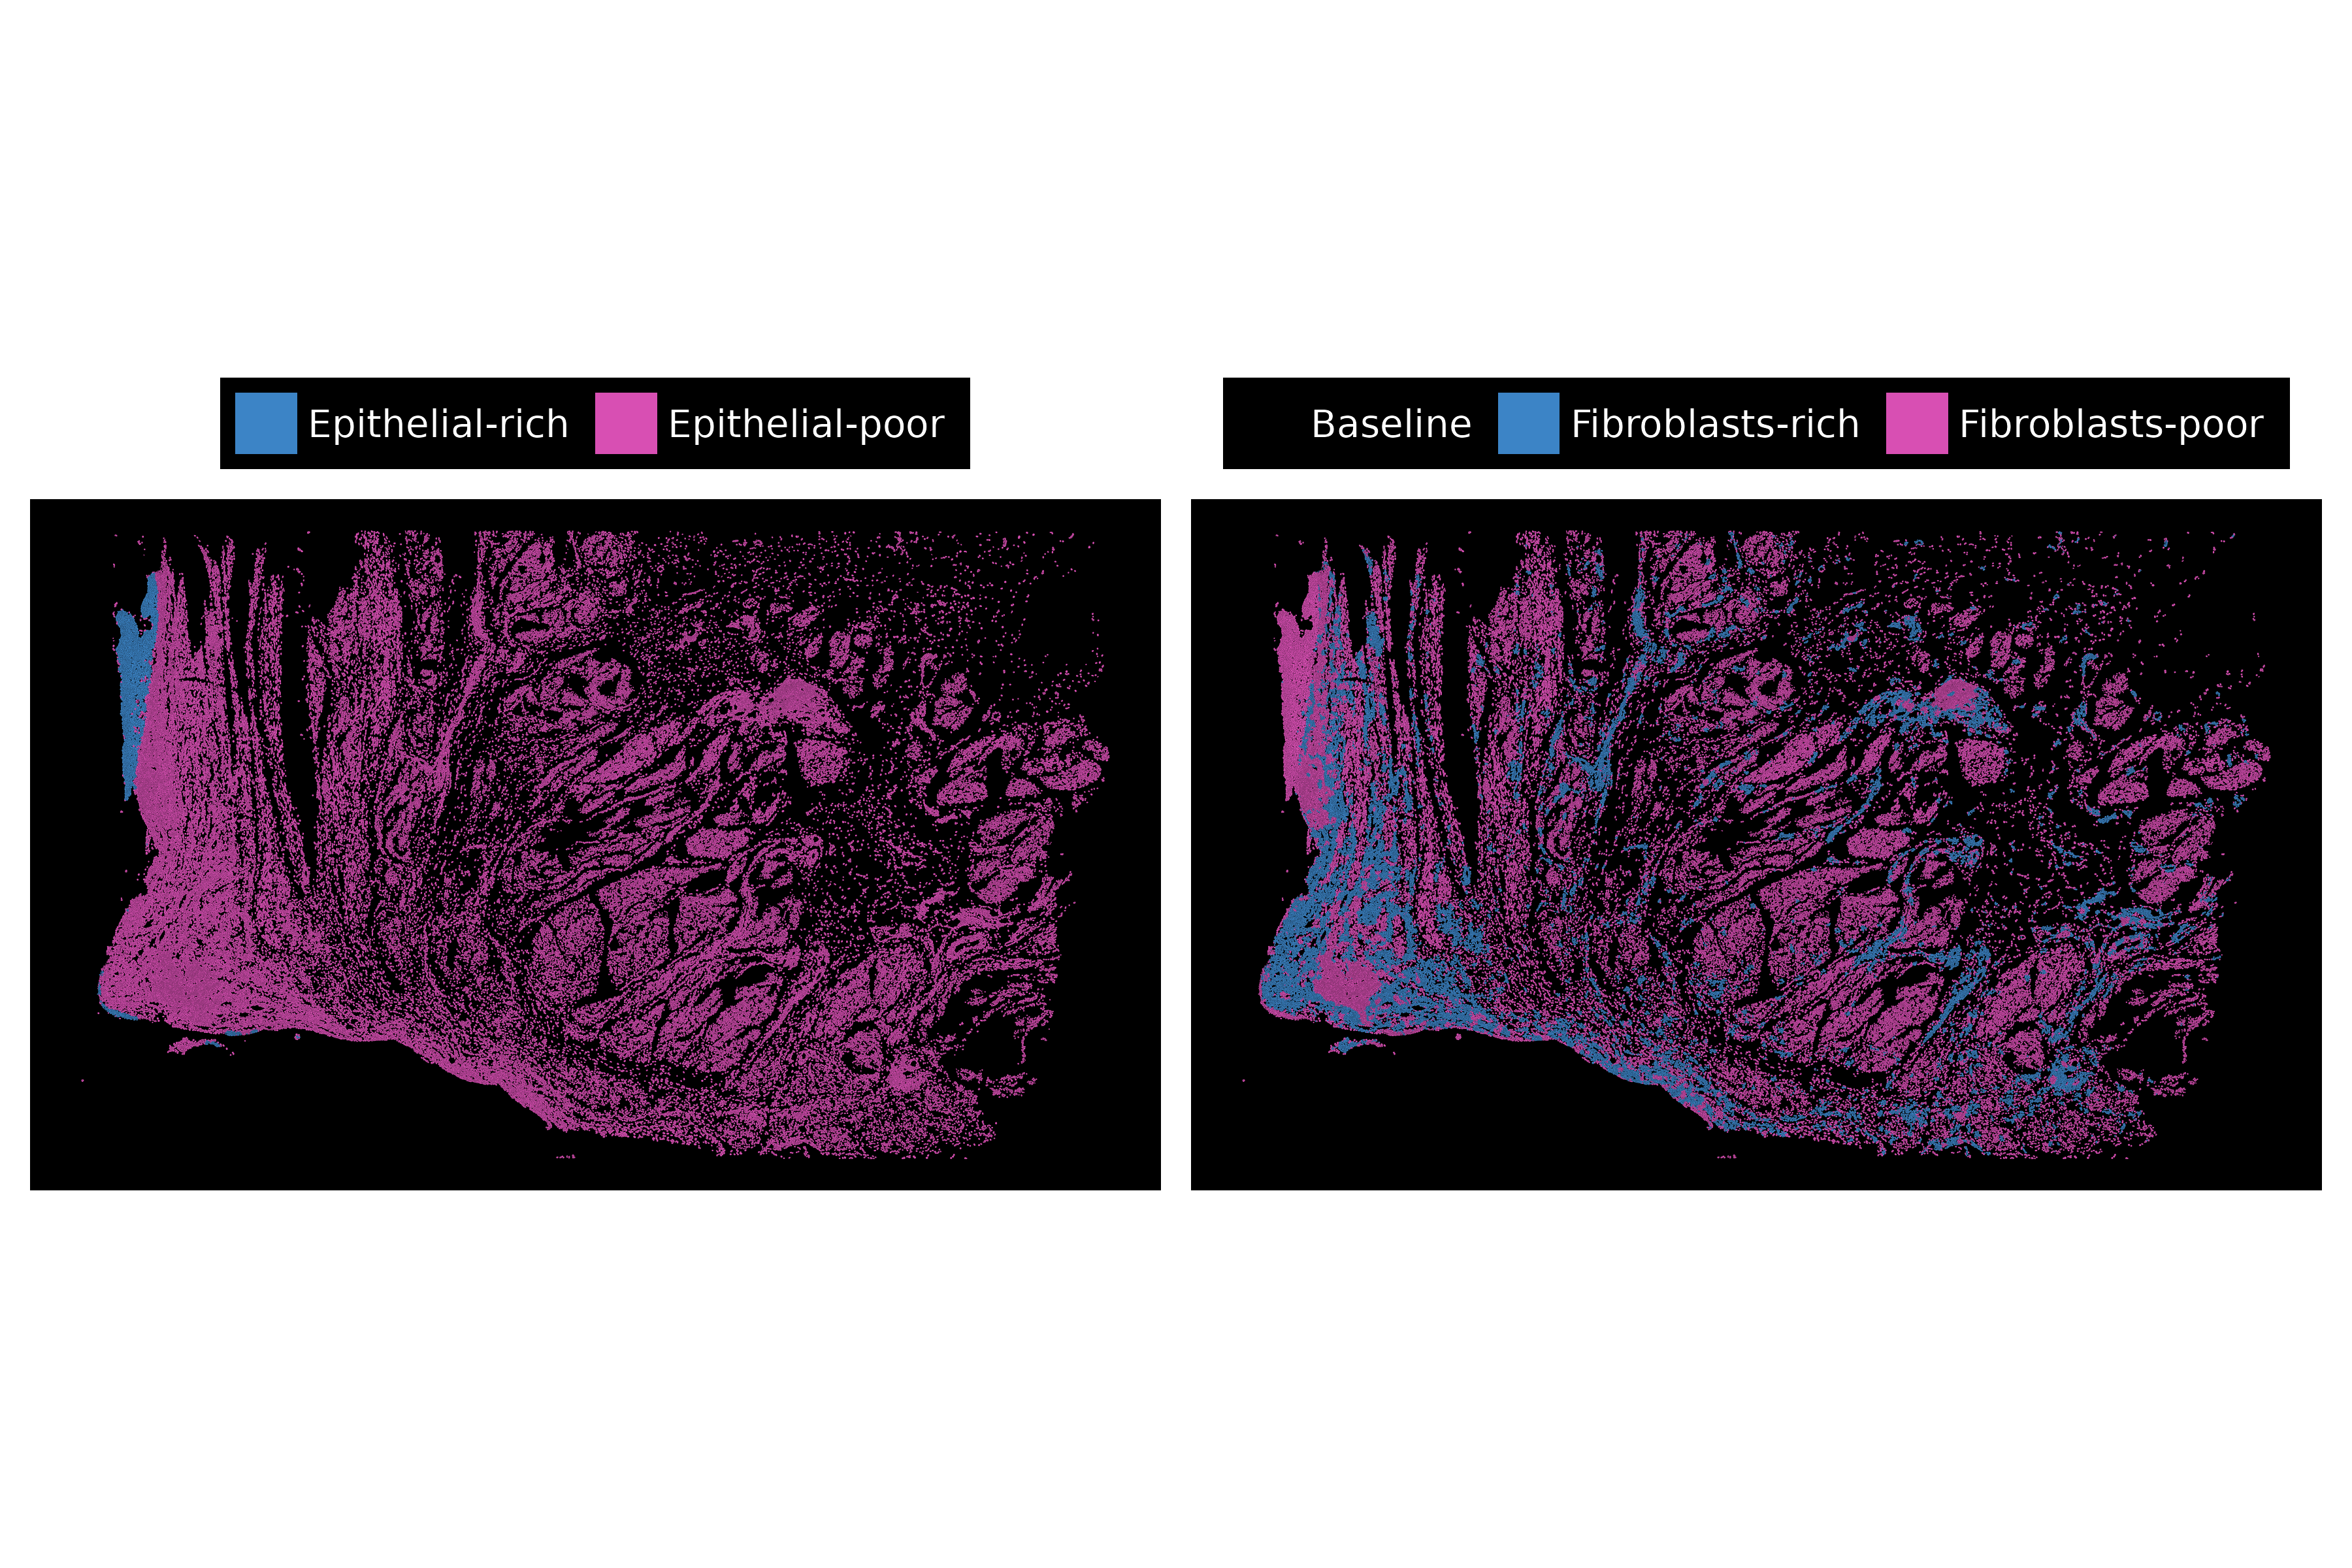
\includegraphics[width=\textwidth]{images/RichPoor_Communities_DU76.png}
    \caption{Spatial distribution of enriched and depleted neighbourhood-defined communities in sample DU76. The left panel shows the localization of epithelial-rich communities, while the right panel displays fibroblast-rich and fibroblast-poor communities projected onto the tissue coordinates.}
    \labfig{Rich_Poor_tissue76}
\end{figure}


As mentioned previously, the spatial organization of the identified communities suggested potential differences between responders and non-responders. However, these observations were based on the qualitative inspection of community architecture and therefore required statistical validation. To quantitatively assess which compositional features were associated with treatment outcome across the available samples, Cohen's *d* effect size was calculated for the relative abundance of each cell type within each cell-rich community, comparing responders and non-responders to immune checkpoint inhibitor (ICI) therapy. In contrast to the previous analyses, which focused on the overall spatial arrangement of communities within the tissue, this approach evaluated whether specific cell populations were differentially represented within each community according to treatment response. 

\begin{figure}[H]
    \centering
    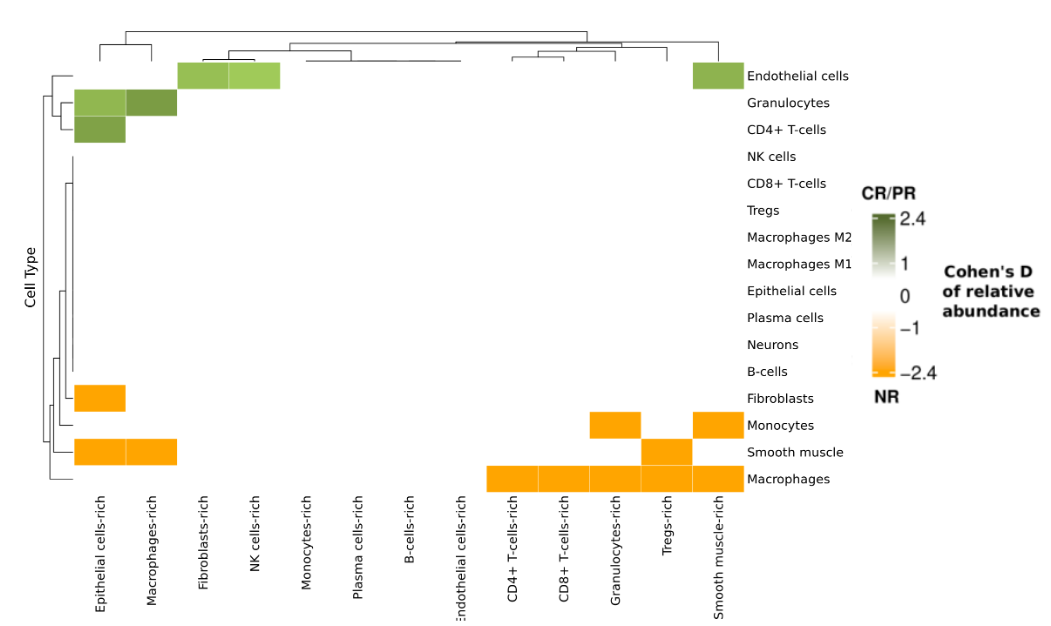
\includegraphics[width=\textwidth]{images/COHENSD_DUTRENEO.png}
    \caption{Heatmap showing Cohen’s D of the relative abundance of each cell type in each cell-rich community, comparing the two response groups among cases from the ICI treatment Xenium cohort. Higher Cohen’s D (dark green color) indicates a higher relative abundance of a given cell type in each community in responders, whereas a higher value towards the orange color indicates the opposite.}
    \labfig{COHENSD_DUTRENEO}
\end{figure}


As shown in \reffig{COHENSD_DUTRENEO}, Cohen's *d* analysis revealed a marked enrichment of fibroblasts within epithelial-rich communities in non-responders from the ICI-treated cohort. Fibroblasts are major regulators of the extracellular matrix and have been implicated in the establishment of immune-excluded tumour phenotypes. Their increased presence surrounding tumour epithelial regions suggests the existence of a stromal-rich microenvironment that may act as a physical and biochemical barrier to immune-cell infiltration. Consequently, even when the immune system is activated through checkpoint blockade with durvalumab and tremelimumab, activated lymphocytes may be unable to efficiently access tumour nests. These findings suggest that, although tumours may display inflammatory signatures such as a high TIS, inflammation alone may not be sufficient to predict response if the spatial organization of the tumour microenvironment limits effective tumour–immune cell interactions.


\begin{figure}[H]
    \centering
    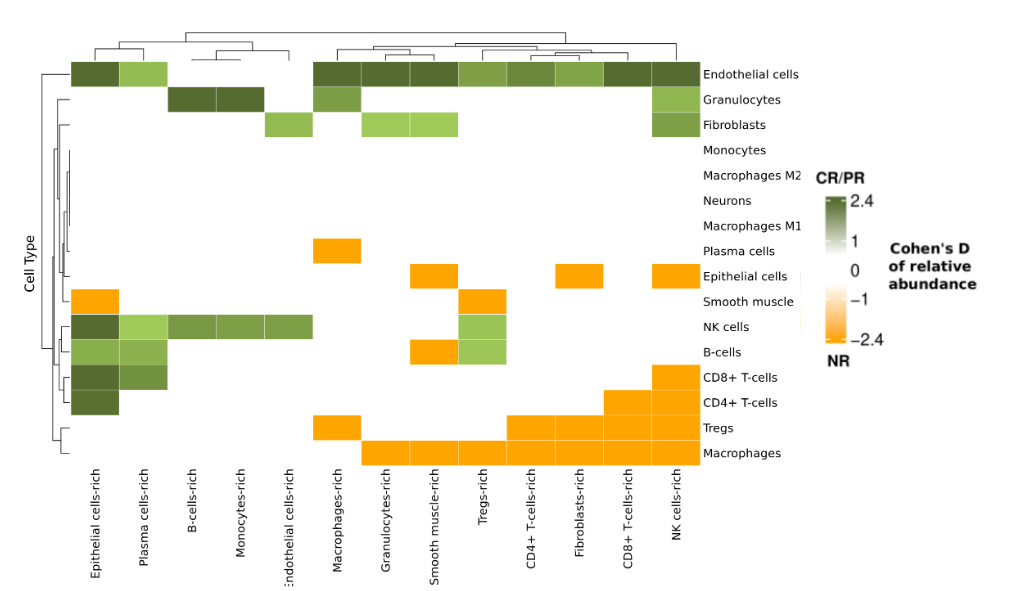
\includegraphics[width=\textwidth]{images/COHENSD_STANDARD.png}
    \caption{Heatmap showing Cohen’s D of the relative abundance of each cell type in each cell-rich community, comparing the two response groups among cases from the standard treatment Xenium cohort. Higher Cohen’s D (dark green color) indicates a higher relative abundance of a given cell type in each community in responders, whereas a higher value towards the orange color indicates the opposite.}
    \labfig{COHENSD_STANDARD}
\end{figure}


The same analysis was performed for the standard neoadjuvant chemotherapy (NAC) cohort (\reffig{COHENSD_STANDARD}). In this case, the association between fibroblast-rich epithelial communities and treatment failure was unexistent. Given that cisplatin-based chemotherapy acts primarily through direct cytotoxic effects rather than immune activation, stromal-mediated immune exclusion would be expected to have a limited impact on treatment efficacy. The stronger association observed in the ICI cohort therefore suggests that immune exclusion may specifically impair therapies that rely on effective anti-tumour immune responses. Together, these results support the hypothesis that stromal-mediated immune exclusion may represent one mechanism underlying the limited predictive value of TIS observed in the DUTRENEO clinical trial.


